%%%%%%%%%%%%%%%%%%%%%%%%%%%%%%%%%%%%%%%%%%%%%%%%%%%%%%%%%%%%%%%%%%%%%%%%%%%%%%%%
%% Plantilla de memoria en LaTeX para la ETSIT - Universidad Rey Juan Carlos
%%
%% Por Gregorio Robles <grex arroba gsyc.urjc.es>
%%     Grupo de Sistemas y Comunicaciones
%%     Escuela Técnica Superior de Ingenieros de Telecomunicación
%%     Universidad Rey Juan Carlos
%% (muchas ideas tomadas de Internet, colegas del GSyC, antiguos alumnos...
%%  etc. Muchas gracias a todos)
%%
%% La última versión de esta plantilla está siempre disponible en:
%%     https://github.com/gregoriorobles/plantilla-memoria
%%
%% Para obtener PDF, ejecuta en la shell:
%%   make
%% (las imágenes deben ir en PNG o JPG)

%%%%%%%%%%%%%%%%%%%%%%%%%%%%%%%%%%%%%%%%%%%%%%%%%%%%%%%%%%%%%%%%%%%%%%%%%%%%%%%%

\documentclass[a4paper, 12pt]{book}
%\usepackage[T1]{fontenc}

\usepackage[a4paper, left=2.5cm, right=2.5cm, top=3cm, bottom=3cm]{geometry}
\usepackage{times}
\usepackage[utf8]{inputenc}
%\usepackage[latin1]{inputenc}
%\usepackage[spanish]{babel} % Comenta esta l�nea si tu memoria es en ingl�s
\usepackage{url}
%\usepackage[dvipdfm]{graphicx}
\usepackage{graphicx}
\usepackage{float}  %% H para posicionar figuras
\usepackage[breaklinks=true]{hyperref} %% Para marcadores
\usepackage[nottoc, notlot, notlof, notindex]{tocbibind} %% Opciones de �ndice
\usepackage{latexsym}  %% Logo LaTeX
\usepackage{csquotes}  %% Paquete para citas (displayquote)
\usepackage{amsthm}  %% Paquete para Teoremas
\usepackage{color}  %% Paquete para texto en color
\usepackage[normalem]{ulem}  %% Para tablas
\useunder{\uline}{\ul}{}  %% Para tablas
\usepackage{listings}  %% para código y comandos
\usepackage{pdfpages}  %% para incluir archivos PDF
\usepackage{enumerate}  %% Para enumerar
\usepackage[parfill]{parskip}  %% Párrafos
\definecolor{codegreen}{rgb}{0,0.6,0}
\definecolor{codegray}{rgb}{0.5,0.5,0.5}
\definecolor{codepurple}{rgb}{0.58,0,0.82}
\definecolor{backcolour}{rgb}{0.82,0.82,0.82}

\lstdefinestyle{mystyle}{
    backgroundcolor=\color{backcolour},
    commentstyle=\color{codegreen},
    keywordstyle=\color{magenta},
    numberstyle=\tiny\color{codegray},
    stringstyle=\color{codepurple},
    basicstyle=\ttfamily\footnotesize,
    breakatwhitespace=false,
    breaklines=true,
    captionpos=b,
    keepspaces=true,
    numbers=left,
    numbersep=5pt,
    showspaces=false,
    showstringspaces=false,
    showtabs=false,
    tabsize=2
}

\lstdefinestyle{mystylesmall}{
    backgroundcolor=\color{backcolour},
    commentstyle=\color{codegreen},
    keywordstyle=\color{magenta},
    numberstyle=\tiny\color{codegray},
    stringstyle=\color{codepurple},
    basicstyle=\ttfamily\scriptsize,
    breakatwhitespace=false,
    breaklines=true,
    captionpos=b,
    keepspaces=true,
    numbers=left,
    numbersep=5pt,
    showspaces=false,
    showstringspaces=false,
    showtabs=false,
    tabsize=2
}

\lstset{style=mystyle}

\title{Memoria del Proyecto}
\author{Miguel Ángel Fernández Sánchez}

\renewcommand{\baselinestretch}{1.5}  %% Interlineado

\begin{document}

%\renewcommand{\refname}{Bibliografía}  %% Renombrando
%\renewcommand{\appendixname}{Apéndice}

%%%%%%%%%%%%%%%%%%%%%%%%%%%%%%%%%%%%%%%%%%%%%%%%%%%%%%%%%%%%%%%%%%%%%%%%%%%%%%%%
% PORTADA

\begin{titlepage}
\begin{center}
\begin{tabular}[c]{c c}
%\includegraphics[bb=0 0 194 352, scale=0.25]{logo} &
\includegraphics[scale=0.25]{img/logo_vect.png} &
\begin{tabular}[b]{l}
\Huge
\textsf{UNIVERSIDAD} \\
\Huge
\textsf{REY JUAN CARLOS} \\
\end{tabular}
\\
\end{tabular}

\vspace{3cm}

\Large
GRADO INGENIERÍA SISTEMAS AUDIOVISUALES Y MULTIMEDIA

\vspace{0.4cm}

\large
Curso Académico 2017/2018

\vspace{0.8cm}

Trabajo Fin de Grado

\vspace{2.5cm}

\LARGE
HERRAMIENTA PARA ANALIZAR PROYECTOS FLOSS EN GITHUB
% http://dl.acm.org/citation.cfm?id=2976778
\vspace{4cm}

\large
Autor : Miguel Ángel Fernández Sánchez \\
Tutor : Dr. Gregorio Robles
\end{center}
\end{titlepage}

\newpage
\mbox{}
\thispagestyle{empty} % para que no se numere esta pagina


%%%%%%%%%%%%%%%%%%%%%%%%%%%%%%%%%%%%%%%%%%%%%%%%%%%%%%%%%%%%%%%%%%%%%%%%%%%%%%%%
%%%% Para firmar
\clearpage
\pagenumbering{gobble}
\chapter*{Evaluation}

\vspace{-4cm}
\begin{center}
\LARGE
\textbf{Trabajo Fin de Grado}

\vspace{1cm}
\large
Herramienta para analizar proyectos FLOSS en GitHub

\vspace{1cm}
\large
\textbf{Autor :} Miguel Ángel Fernández Sánchez \\
\textbf{Tutor :} Dr. Gregorio Robles Martínez

\end{center}

\vspace{1cm}
La defensa del presente Trabajo Fin de Grado se realizó el día \qquad$\;\,$ de \qquad\qquad\qquad\qquad \newline de 2018, siendo calificada por el siguiente tribunal:


\vspace{0.5cm}
\textbf{Presidente:}

\vspace{1.2cm}
\textbf{Secretario:}

\vspace{1.2cm}
\textbf{Vocal:}


\vspace{1.2cm}
y habiendo obtenido la siguiente calificación:

\vspace{1cm}
\textbf{Calificación:}


\vspace{1cm}
\begin{flushright}
Fuenlabrada, a \qquad$\;\,$ de \qquad\qquad\qquad\qquad de 2018
\end{flushright}

%%%%%%%%%%%%%%%%%%%%%%%%%%%%%%%%%%%%%%%%%%%%%%%%%%%%%%%%%%%%%%%%%%%%%%%%%%%%%%%%
%%%% Dedicatoria

\chapter*{Dedications}
\pagenumbering{Roman} % para comenzar la numeracion de paginas en numeros romanos
\begin{flushright}
\textit{A mi madre y a mi padre:\\
Esta memoria no hubiera sido posible \\
sin vuestro incansable esfuerzo y apoyo.}
\end{flushright}
\par
\begin{flushright}
\textit{A mi hermana, Ana:\\
Con esfuerzo y constancia,\\
alcanzarás todo lo que te propongas.\\}
\end{flushright}
\begin{flushright}
\textit{\\To my mother and father:\\
This thesis wouldn't have been possible\\
without your endless effort and support.}
\end{flushright}
\par
\begin{flushright}
\textit{To my sister, Ana:\\
With effort and persistence,\\
you will reach all of your goals.}
\end{flushright}
%%%%%%%%%%%%%%%%%%%%%%%%%%%%%%%%%%%%%%%%%%%%%%%%%%%%%%%%%%%%%%%%%%%%%%%%%%%%%%%%
%%%% Agradecimientos

\chapter*{Acknowledgements}
%\addcontentsline{toc}{chapter}{Agradecimientos} % si queremos que aparezca en el �ndice
\markboth{ACKNOWLEDGEMENTS}{ACKNOWLEDGEMENTS} % encabezado

First, I want to thank my parents and the rest of my family. Their constant effort and support
along with the values they taught me, made possible for me studying at the university. These words
are dedicated to them: This is your success, I love you.\par
I want to thank my tutor Gregorio, for believing in me, and giving me the great opportunity of working
in LibreSoft research group where I've lived some of my great experiences at the university;
growing as a person, meeting wonderful people, travelling and learning far beyond I could have ever imagined.\par
To my friends and classmates from the university: Eva, Eduardo, Bea, Diego, Olalla, Raúl, Sara, Luismi, Javi, Marta, Dani, Carol,
Celia, Nuria, Vanessa, Raquel and many, many more. Without your friendship, help and support I wouldn't reached this goal, thank you.\par
To the people who has helped me to review and improve this thesis: Gregorio, Santi, Valerio, Fernando, Saray, Eva and Sara. Thank you
for your patience and sharing your time and knowledge so generously.\par
Finally, thank to the people who contributed with their GitHub account to make this study possible:
Gregorio R., Michel C., Truong H.Q., Eva H., Olalla S., Beatriz C., Diego S.,
Eduardo D., Javier M., Diego J., Jose M., Alejandro F., Ángel C., Alejandro, Cristina, Fernando, Irene, Nacho, Ana R. y Ronny.
%%%%%%%%%%%%%%%%%%%%%%%%%%%%%%%%%%%%%%%%%%%%%%%%%%%%%%%%%%%%%%%%%%%%%%%%%%%%%%%%
%%%% Resumen en ingl�s
\chapter*{Summary}
%\addcontentsline{toc}{chapter}{Summary} % si queremos que aparezca en el �ndice
\markboth{SUMMARY}{SUMMARY} % encabezado

Here comes a translation of the ``Resumen'' into English. Please, double check
it for correct grammar and spelling. As it is the translation of the ``Resumen'',
which is supposed to be written at the end, this as well should be filled out
just before submitting.


%%%%%%%%%%%%%%%%%%%%%%%%%%%%%%%%%%%%%%%%%%%%%%%%%%%%%%%%%%%%%%%%%%%%%%%%%%%%%%%%
%%%% Resumen

\chapter*{Resumen}
%\addcontentsline{toc}{chapter}{Resumen} % si queremos que aparezca en el �ndice
\markboth{RESUMEN}{RESUMEN} % encabezado

Aquí viene un resumen del proyecto. Ha de constar de tres o cuatro párrafos,
donde se presente de manera clara y concisa de qué va el proyecto. Han
de quedar respondidas las siguientes preguntas:

\begin{itemize}
  \item ¿De qué va este proyecto? ¿Cuál es su objetivo principal?
  \item ¿Cómo se ha realizado? ¿Qué tecnologías están involucradas?
  \item ¿En qué contexto se ha realizado el proyecto? ¿Es un proyecto
dentro de un marco general?
\end{itemize}
Lo mejor es escribir el resumen al final.
%%%%%%%%%%%%%%%%%%%%%%%%%%%%%%%%%%%%%%%%%%%%%%%%%%%%%%%%%%%%%%%%%%%%%%%%%%%%%%%%
%%%%%%%%%%%%%%%%%%%%%%%%%%%%%%%%%%%%%%%%%%%%%%%%%%%%%%%%%%%%%%%%%%%%%%%%%%%%%%%%
% �NDICES %
%%%%%%%%%%%%%%%%%%%%%%%%%%%%%%%%%%%%%%%%%%%%%%%%%%%%%%%%%%%%%%%%%%%%%%%%%%%%%%%%

% Las buenas noticias es que los �ndices se generan autom�ticamente.
% Lo �nico que tienes que hacer es elegir cu�les quieren que se generen,
% y comentar/descomentar esa instrucci�n de LaTeX.

%%%% �ndice de contenidos
\tableofcontents
%%%% �ndice de figuras
\cleardoublepage
%\addcontentsline{toc}{chapter}{Lista de figuras} % para que aparezca en el indice de contenidos
\listoffigures % indice de figuras
%%%% �ndice de tablas
%\cleardoublepage
%\addcontentsline{toc}{chapter}{Lista de tablas} % para que aparezca en el indice de contenidos
%\listoftables % indice de tablas

%%%%%%%%%%%%%%%%%%%%%%%%%%%%%%%%%%%%%%%%%%%%%%%%%%%%%%%%%%%%%%%%%%%%%%%%%%%%%%%%
%%%%%%%%%%%%%%%%%%%%%%%%%%%%%%%%%%%%%%%%%%%%%%%%%%%%%%%%%%%%%%%%%%%%%%%%%%%%%%%%
% INTRODUCCI�N %
%%%%%%%%%%%%%%%%%%%%%%%%%%%%%%%%%%%%%%%%%%%%%%%%%%%%%%%%%%%%%%%%%%%%%%%%%%%%%%%%

\cleardoublepage
\chapter{Introduction}
\label{sec:intro} % etiqueta para poder referenciar luego en el texto con ~\ref{sec:intro}
\pagenumbering{arabic} % para empezar la numeraci�n de p�gina con n�meros
% En este cap�tulo se introduce el proyeto. Deber�a tener informaci�n general sobre
% el mismo, dando la informaci�n sobre el contexto en el �que se ha desarrollado.
% No te olvides de echarle un ojo a la p�gina con los cinco errores de escritura m�s frecuentes\footnote{\url{http://www.tallerdeescritores.com/errores-de-escritura-frecuentes}}.
% #TODO Ask for resources to back this data:
GitHub is the most used online code platform in the world. We can extract huge amounts of information from millions of projects
about how is the software being developed: productivity, issue-tracking methods, developer-to-developer relations, etc. [RGBM06]
For researchers, GitHub is an endless source of publicly available data for potential studies, and for companies and communities
is probably the best way to know deeply how its software is evolving over time, so they can use this data to make the right decisions
for the future (known as data-driven decisions).\par
I was working as a researcher assistant in \emph{GSyC/LibreSoft}\footnote{\url{http://www.libresoft.es}} department at
Rey Juan Carlos University when I started to deepen into Free/Libre software and the world of metrics.
Then I had the great luck of start participating in a study that
Dr. Gregorio Robles was doing with researchers from Chalmers University in Gothenburg, Sweden. The main aim of their research was to
learn how \emph{UML} models\footnote{\url{http://uml.org/what-is-uml.htm}} are used in public
\emph{FLOSS}\footnote{Free/Libre and Open Source Software. Complete definition at section~\ref{sec:floss-definition}} projects
(particularly, projects hosted on GitHub), as most of the previous studies focused only on its industrial use.\\
Given the large size of GitHub as a platform and its access limitations, this research motivated to build a tool which extracts
Git data from all the existing repositories on GitHub, then filter those repositories which may include at least one
\emph{UML} model and finally analyze more in-depth the set of projects that meet this condition.\par
Since early stages of this research, this tool was designed and built using a modular structure, thought to be reusable
and adaptable to any kind of files that have to be found but also the way GitHub provides data; hoping to be useful
for other researches or any other person who might be interested on extracting this information. Besides, the scale of this project
presented a personal challenge which provided me the opportunity to extend my knowledge and obtain a valuable point of
view about research and large-scope projects.
\section{Context}
\label{sec:context}
The way people develop software has evolved during these years. There is an extended social perception of developers to
being introverted, solitary people, with very few social skills, but this sense is outdated: the paradigm has changed,
as coding has become a social activity. Developers who work collaborating with others produce better software [resource], as they
are continuously reading code from other developers, getting feedback about their contributions and consequently
widening their knowledge with new procedures and ideas.\par
In the last few years we have seen how this social trend came to software with the
emergence of social coding platforms, such as GitHub\footnote{\url{https://github.com}},
BitBucket\footnote{\url{https://bitbucket.org/product}}, GitLab\footnote{\url{https://gitlab.com/}}, etc.\\
Social interactions in these platforms are about how software is developed and maintained but also how
contributions are managed (code review, continuous integration, etc.).\\
So, for example, on GitHub\footnote{\url{https://github.com}} we can interact to obtain or produce different data:
\begin{itemize}
    \item \textit{Forking} a repository (create an editable copy of a project).
    \item Comparing the changes from last \textit{commit} (difference between most recent version and last version of the project).
    \item Contributing to a repository.
    \item Submitting a \textit{Pull Request} (proposal to merge changes in a project).
\end{itemize}
These interactions that were mentioned leave traces which remain stored in some computer on Earth and generally
they are visible to everybody.
This means we can obtain these data (though not all of it is publicly available) through the Internet using an
\emph{API}\footnote{See the definition for API in section~\ref{sec:api}}.\\
Once this information is retrieved, we can analyze it and extract conclusions about it.\par
To complete the context for this thesis is necessary to situate what UML is and why it is important.
The Universal Modeling Language (UML) is a graphic, descriptive language to visualize, specify, construct and document the
artifacts from a system (mainly; structure, behavior and interaction) containing a great amount of software.
UML provides a standard way to write the plans of a system, covering from conceptual aspects like business processes and
system features to particular aspects like classes from a certain programming language, database schemas and reusable
software components with a higher level of abstraction. Therefore, modelling with UML is considered as one more component
in a software development process.\par
For industrial software, the use of UML is commonly accepted and software engineering researchers in the area of modeling
have made efforts to collect examples of projects that use modelling and their models. Nonetheless, industrial projects
are very averse to share their models because of these projects licenses and privacy issues (For instance; its current
state, new features, etc.).
This situation hinders the task of creating a models data-set for researchers, who had achieved in summer 2016 a data-set
containing around 81 models from open source projects. At this moment, there was not much research about the use of UML in open source.
Furthermore, most open source code platforms do not provide any feature for model management, which made researchers think that UML
is not very frequent in FLOSS projects.
Still, there was no quantification of its occurrence.\par
In this context, a tandem research was born uniting the experience of LibreSoft team researchers (from Rey Juan Carlos University) about
FLOSS and software development processes and the experience of Software Engineering division team researchers (from Chalmers University)
about software modelling to obtain quantitative data about the use of UML in open source projects. To make this study a reality, they
decided to get these projects from GitHub because is the code platform containing the greatest amount of FLOSS projects.
This was the motivation to create the tool presented in this thesis, to perform a systematic search looking for UML models in
an automated and scalable way.\\
As I explain in the ``Results'' section (\ref{sec:case-study-uml}), a total of 93.596 publicly available UML models were identified thank to this research.
This amount of models compounds a data-set that is two orders of magnitude larger than the previous UML data-sets from previous studies. The results
obtained with this tool and its subsequent analysis led to several scientific papers published on international Software Engineering conferences,
as I detail on section~\ref{sec:results}. These published papers are available on appendix~\ref{app:papers}.
\section{Free/Libre/Open-Source Software}
\label{sec:floss-definition}
The tool presented in this thesis is distributed as Free/Libre software. Moreover, in the following sections we are going
to talk about software and its development process, focusing on Free/Libre and Open-source
software (\emph{FLOSS}) projects, therefore it is inevitable to describe briefly what this is about.\par
According to the \textbf{Free Software Foundation}\footnote{\url{https://www.gnu.org/philosophy/free-sw.html}}:
\begin{displayquote}
    \emph{Free software} means software that respects users' freedom and community. Roughly, it means that the users have the freedom
    to run, copy, distribute, study, change and improve the software. Thus, free software is a matter of liberty, not price. (\ldots)
    (For an extended definition, see section~\ref{sec:freedoms}).\\
\end{displayquote}
Due to the connotations which the word \emph{Free} has in English language (mentioned before), there is a definition
for \emph{Open source} software by the \textbf{Open Source Initiative}\footnote{\url{https://opensource.org/osd}} which
slightly varies from the \emph{FSF} definition. About this difference, Richard Stallman (founder of the \emph{FSF}) comments:
\begin{displayquote}
The term \emph{open source} software is used by some people to mean more or less the same category as free software.
It is not exactly the same class of software: they accept some licenses that we consider too restrictive,
and there are free software licenses they have not accepted. However, the differences in extension of the
category are small: nearly all free software is open source, and nearly all open source software is free.
\end{displayquote}
During my degree, I was fortunate to be taught within \emph{FLOSS} values, as most of my professors plead
for Free/Libre software as their teaching model, by which I have obtained a distinctive knowledge and perspective
as a professional but also as an individual.
%%%%%%%%%%%%%%%%%%%%%%%%%%%%%%%%%%%%%%%%%%%%%%%%%%%%%%%%%%%%%%%%%%
\section{Structure of the thesis}
\label{sec:structure}
In this thesis are presented the main objectives which were marked to build this tool in chapter~\ref{sec:objectives} ``Objectives'',
followed by a brief explanation of the technology which have been used to achieve these objectives in chapter~\ref{sec:state-art} ``State of the art''.
Next, in chapter~\ref{sec:design-implementation} ``Design and implementation'' it is detailed the designing process and the tool architecture, itemizing on each one of its components.
Thenceforth, the performance and results of the tool are explored in chapter~\ref{sec:results} ``Results'' by means of two different use cases,
detailing the obtained results but also taking into account the technical particularities which arose during its development and how they were solved.
Furthermore, some conclusions are presented in chapter~\ref{sec:conclusions} ``Conclusions'', reviewing whether the marked objectives have been accomplished or not,
along with a brief discussion about the limitations of this tool and future work.\par
Additionally, this thesis contains the following annexes:
\begin{enumerate}[A.]
  \item Definitions
  \item Main scripts of the tool
  \item User manual
  \item Published papers
\end{enumerate}
%%%%%%%%%%%%%%%%%%%%%%%%%%%%%%%%%%%%%%%%%%%%%%%%%%%%%%%%%%%%%%%%%%%%%%%%%%%%%%%%
%%%%%%%%%%%%%%%%%%%%%%%%%%%%%%%%%%%%%%%%%%%%%%%%%%%%%%%%%%%%%%%%%%%%%%%%%%%%%%%%
% OBJETIVOS %
%%%%%%%%%%%%%%%%%%%%%%%%%%%%%%%%%%%%%%%%%%%%%%%%%%%%%%%%%%%%%%%%%%%%%%%%%%%%%%%%
\cleardoublepage
\chapter{Objectives}
\label{sec:objectives}
This tool was created with the purpose of answering two main research questions:
\begin{itemize}
  \item RQ1: How many GitHub repositories contain at least one file with a certain extension or a certain
        pattern in its file-name?
  \item RQ2: What is the history of those files in the life-span of the project?
\end{itemize}
Thus far, many studies focused in one single project or in a limited data-set when software development is analyzed,
whereas the aim of this research was to obtain the whole data-set of repositories hosted on the GitHub platform
in order to obtain quantitative information about the usage of a certain file type, programming language
or/and any search that can be expressed into patterns and heuristics. Then, store that data in a database
where it can be analyzed in a deeper way to extract elaborate information about the data-set.\par
To meet these requirements, the tool had to achieve the following main objectives:
\begin{itemize}
  \item OB1: Extract the whole set of projects hosted in GitHub.
  \item OB2: Collect data from all public projects about their file structure in a scalable, automated way.
  \item OB3: Establish a procedure to filter this extracted data using a determined kind of heuristics and patterns.
  \item OB4: Analyze positive GitHub repositories (with at least one positive result) to obtain enhanced Git data from them.
  \item OB5: Store this enhanced data in a database whose structure allows to query information of interest.
\end{itemize}
To accomplish OB1 in a proper way we needed an static, reliable and updated source of GitHub.
GitHub allows to obtain its information through its \textit{API},
but this entails several limitations. To mention the most important ones:
\begin{itemize}
    \item The GitHub API has a maximum rate of 5.000 request per hour with each account.
    \item GitHub is not static (new repositories are added, existing ones are modified, etc.) which leads to the problem of
    accessing concurrently to its data.
    \item There isn't a direct way
    of obtaining the amount of repositories in the platform at a certain date using its \textit{API}.
\end{itemize}
These limitations led to the decision of using the \emph{GHTorrent} project, which offers a queriable, offline \emph{MySQL}
database with most of the information which the GitHub API can provide.\par
Although GitHub allows to filter projects by a certain programming language (e.g. \emph{Python}, \emph{C++}, etc.),
it does not offer a mechanism through which you can identify projects containing files with a certain extension or how many files
match with some word or pattern in their file-name in a repository. Therefore, to achieve OB2 and OB3 we need to extract the list of files
from the main branch\footnote{Definition of branch and other Git objects in section~\ref{ssec:git-branch}} of each repository,
but \emph{GHTorrent} data does not contain file-related information, so it is necessary to define a method to access the GitHub API
in order to retrieve this information so later it can be applied a set of filters to determine which repositories meet the established
requirements. Once OB1, OB2 and OB3 are achieved, the obtained results will constitute the answer to RQ1.\par
OB4 and OB5 have to be completed to answer \emph{RQ2}. Analyzing Git repositories is not a trivial task, as it is crucial
to retrieve complete and reliable information from them to perform a robust analysis. That's why it was decided to
use a tool called \emph{Perceval} which belongs to the \emph{GrimoireLab} project, a mature and Free/Libre tool-set for software development
analytics, to comply with OB4. It should be noted that this tool is not valid to perform OB2 and that's why the direct access to the
GitHub API is still needed. Lastly, to accomplish OB5 the approach is to store the data obtained with \emph{Perceval} in a database to execute
the necessary queries to obtain answers for RQ2 and any further questions.
%%%%%%%%%%%%%%%%%%%%%%%%%%%%%%%%%%%%%%%%%%%%%%%%%%%%%%%%%%%%%%%%%%%%%%%%%%%%%%%%
%%%%%%%%%%%%%%%%%%%%%%%%%%%%%%%%%%%%%%%%%%%%%%%%%%%%%%%%%%%%%%%%%%%%%%%%%%%%%%%%
% ESTADO DEL ARTE %
%%%%%%%%%%%%%%%%%%%%%%%%%%%%%%%%%%%%%%%%%%%%%%%%%%%%%%%%%%%%%%%%%%%%%%%%%%%%%%%%
\cleardoublepage
\chapter{State of the art}
\label{sec:state-art}
%Puedes citar libros, como el de Bonabeau et al. sobre procesos estigm�rgicos~\cite{bonabeau:_swarm}.
 % Nota que el ~ a�ade un espacio en blanco, pero no deja que exista un salto de l�nea. Imprescindible ponerlo para las citas.
%%%%%%%%%%%%%%%%%%%%%%%%%%%%%%%%%%%
There are multiple tools to analyze GitHub repositories. Nonetheless, at the moment when this tool was designed
there wasn't one single application capable of meeting at once the different and diverse requirements for the
researcher's needs to complete this study.
The uniqueness of the structure of this information along the process and its scale, together with the advantage of
controlling every stage of this tool in order to ensure the truthfulness of the results, triggered the need of
creating a customized, modular tool to satisfy every aspect of the study as much as possible.\par
These are the technologies that were chosen to build this tool. Every technology will be motivated in the next chapter,
``Design and implementation'':
\section{Python}
\label{sec:python}
\textbf{Python}\footnote{\url{https://www.python.org/}} is an interpreted, object-oriented, high-level, open source
programming language for general-purpose programming created by Guido van Rossum in 1991 (Nowadays, the most
recent version is 3.6.4, from December, 2017).\ Its design is focused on code readability and clear syntax, making
possible to program using fewer lines of code comparing to other programming languages as \emph{C++} or \emph{Ada}.\\
%Python is widely used over the world, for example: Numeric and Scientific Programming, ... \\
\emph{Python} features a large standard library, which includes many different tasks from text pattern matching to network
scripting, in addition to a vast collection of third-party application libraries.
Other remarkable features are portability, as \emph{Python} interpreters are available for many operating systems;
and the component integration, as \emph{Python} scripts can easily communicate with other parts of an application or code,
like \emph{C++} libraries, \emph{MySQL} databases, etc.\\
%As a downside to Python is that its execution speed may not always be as fast as a compiled, lower-level
%slanguages such as C and C++.\\
%%%%%%%%%%%%%%%%%%%%%%%%%%%%%%%%%%%
\section{Git}
\label{sec:git}
%source: https://git-scm.com/book/en/v2/Getting-Started-Git-Basics
\textbf{Git} is an open-source Version Control System (\emph{VCS}), originally developed in 2005 by Linus Torvalds.\
As any \emph{VCS}, \emph{git} is a system that records changes to a file or set of files over time
so that you can recall specific versions later.
It is by far, the most used \emph{VCS} in the world\footnote{\url{http://stackoverflow.com/research/developer-survey-2015}}.\par
The major difference between \emph{git} and any other VCS is the way \emph{git} thinks about its data.
Conceptually, most other systems store information as a list of file-based changes. Other systems like \textit{Subversion},
\textit{Perforce}, \textit{Bazaar}, etc. think of the information they store as a set of files and the changes made to each
file over time (See figure~\ref{fig:info-not-git}).\\
Instead, \emph{git} thinks of its data more like a series of snapshots of a miniature file-system (See figure~\ref{fig:info-git}).
With \emph{git}, every time you commit or save the state of your project, \emph{git} basically takes a picture of what all
your files look like at that moment and stores a reference to that snapshot. To be efficient, if files have not changed,
\emph{git} doesn't store the file again, just a link to the previous identical file it has already stored.
All this information is stored in a key-value system as \emph{git} objects, with a unique identity for each of them.
\begin{figure}
  \centering
  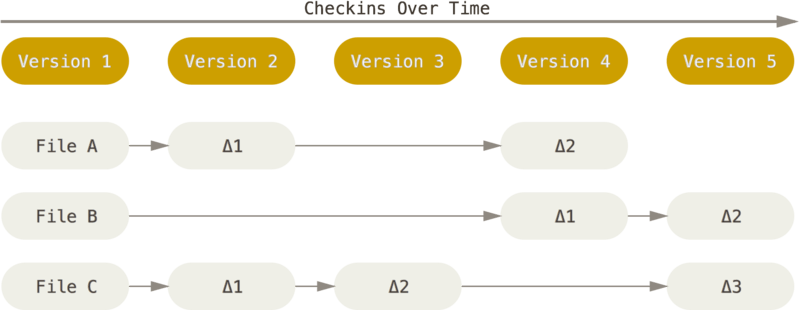
\includegraphics[width=12cm, keepaspectratio]{img/deltas-not-git}
  \caption{How other non-\emph{git} \emph{VCS} store information (Source: Git documentation).}
  \label{fig:info-not-git}
\end{figure}
\begin{figure}
  \centering
  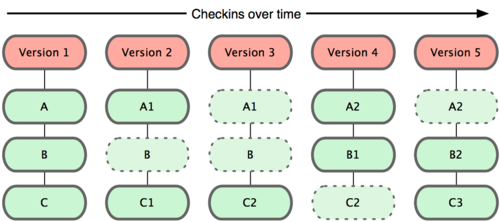
\includegraphics[width=12cm, keepaspectratio]{img/snapshots-git}
  \caption{How \emph{git} structures its information internally (Source: Git documentation).}
  \label{fig:info-git}
\end{figure}
%%%%%%%%%%%%%%%%%%%%%%%%%%%%%%%%%%%
\section{GitHub}
\label{sec:github}
\textbf{GitHub} is a \emph{git}, web-based repository hosting service founded back in 2008. While \emph{git} is a command
line tool, GitHub provides a graphical interface, adding its own collaboration features such as a wikis and basic task
management tools for every project.\\
Each user on GitHub has their own profile, showing its past work and contributions to
other projects via \textit{pull requests}, \textit{forking} (create editable copies into someone's account) other repositories, etc.
Project revisions can be discussed publicly via \textit{issues} so many people can collaborate together to advance a project
forward. GitHub is currently the largest host of source code in the world (See figure~\ref{fig:total-repo-number} for a quantitative
estimation of its scale evolution across time).
% # TODO: https://growthhackers.com/growth-studies/github, https://blog.github.com/2013-12-23-10-million-repositories/
\begin{figure}
  \centering
  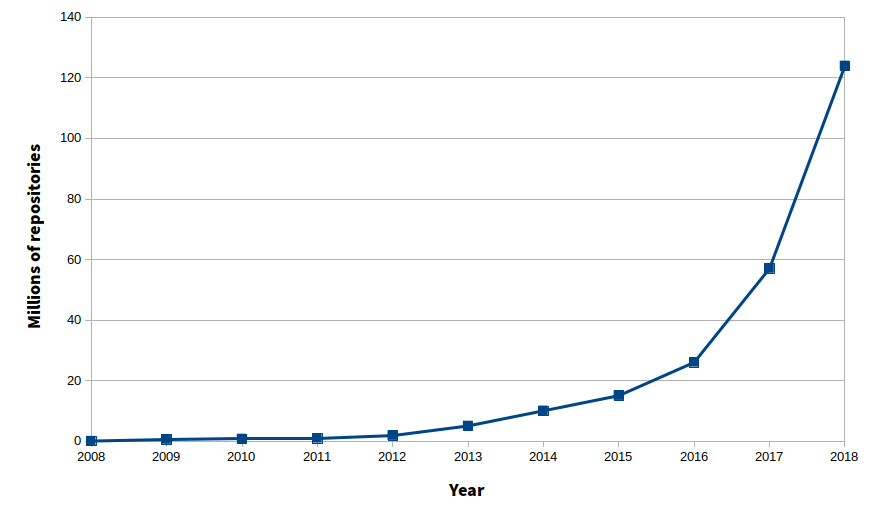
\includegraphics[width=14cm, keepaspectratio]{img/number-github-repos}
  \caption{Evolution of number of repositories on GitHub across time}
  \label{fig:total-repo-number}
\end{figure}
% TODO: https://www.quora.com/How-many-repositories-are-there-on-GitHub
%       https://www.howtogeek.com/180167/htg-explains-what-is-github-and-what-do-geeks-use-it-for/
%       https://techcrunch.com/2012/07/14/what-exactly-is-github-anyway/
%%%%%%%%%%%%%%%%%%%%%%%%%%%%%%%%%%%
\section{GHTorrent}
\label{sec:ghtorrent}
\textbf{GHTorrent} is a project based on create a scalable, queriable, offline mirror of data offered through the GitHub \textit{API}.\\
As they explain in their website\footnote{\url{http://ghtorrent.org/}}, \emph{GHTorrent} monitors the GitHub public event time line.
For each event, it retrieves its contents and their dependencies, exhaustively. Then, it stores the raw responses to a database whose
structure is represented in figure~\ref{fig:ghtorrent-schema}.\
For each release, you can choose the \textit{dump} (a raw copy of a database) you want to download: either a \emph{MySQL} dump
(the full database, using one file per table) or a \emph{MongoDB} one (an incremental database).
\begin{figure}
  \centering
  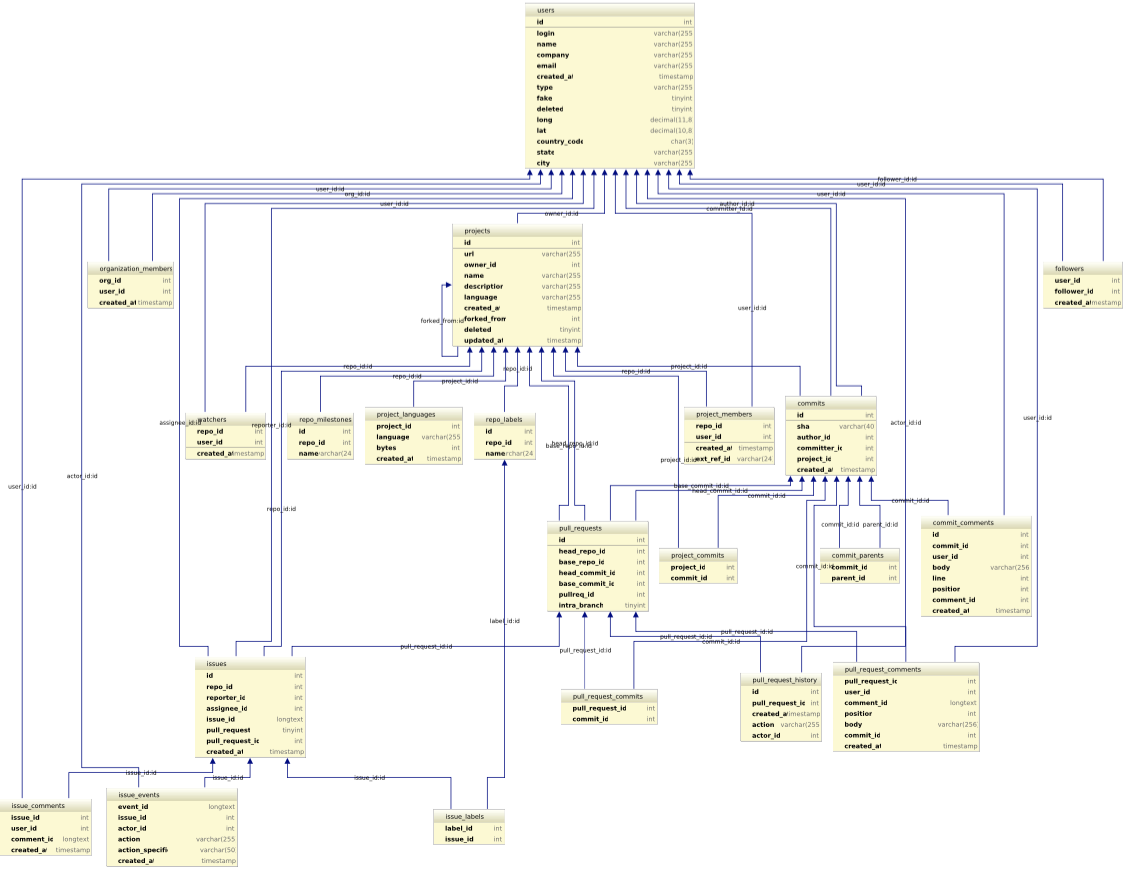
\includegraphics[width=16cm, keepaspectratio]{img/ghtorrent-schema}
  \caption{GHTorrent database relational schema}
  \label{fig:ghtorrent-schema}
\end{figure}
%%%%%%%%%%%%%%%%%%%%%%%%%%%%%%%%%%%
\section{GrimoireLab and Perceval}
\label{sec:grimoire}
\textbf{GrimoireLab}\footnote{\url{http://grimoirelab.github.io/}} is a free, open source tool-set for software development analytics
mainly developed by the Spanish company \emph{Bitergia}\footnote{\url{https://bitergia.com/}}.
It allows you to retrieve data from many kinds of systems with information related to software development, and produce
analysis and visualizations with it.\\
We are focusing on a particular tool of \emph{GrimoireLab} called \textbf{Perceval}. This tool can retrieve data from more
than 20 different kinds of data sources, from \emph{git} repositories or GitHub projects, to issue trackers such as \emph{Jira}
or \emph{Bugzilla}, including messaging systems such as \emph{IRC}, \emph{Slack} or mailing lists, or other types of systems such as
\emph{StackOverflow} or \emph{Jenkins} in a regular and incremental way, allowing to produce uniform sets of information.
\newline \emph{GrimoireLab} is now part of \emph{CHAOSS}\footnote{\url{https://chaoss.community/}}, a project by \emph{The Linux Foundation}.
%%%%%%%%%%%%%%%%%%%%%%%%%%%%%%%%%%%
\section{MySQL}
\textbf{MySQL} is an open-source relational database management system based on Structured Query Language (SQL),
which is the most popular language for adding, accessing and managing content in a database. It is most noted for its quick processing,
proven reliability, ease and flexibility of use.\par
MySQL works in multiple platforms, running as a server and allows multiple users (MySQL \emph{clients}) to manage and create numerous databases.
It is a central component in the LAMP stack of open source web application
software (LAMP stands for Linux, Apache, MySQL, and PHP) and it is adequate to be used in high-profile, large-scale systems and websites.
To mention some examples, MySQL is used by Facebook, Twitter, Flickr and YouTube.
%%%%%%%%%%%%%%%%%%%%%%%%%%%%%%%%%%%%%%%%%%%%%%%%%%%%%%%%%%%%%%%%%%%%%%%%%%%%%%%%
%%%%%%%%%%%%%%%%%%%%%%%%%%%%%%%%%%%%%%%%%%%%%%%%%%%%%%%%%%%%%%%%%%%%%%%%%%%%%%%%
% DISEÑO E IMPLEMENTACIÓN %
%%%%%%%%%%%%%%%%%%%%%%%%%%%%%%%%%%%%%%%%%%%%%%%%%%%%%%%%%%%%%%%%%%%%%%%%%%%%%%%%
\cleardoublepage
\chapter{Design and implementation}
\label{sec:design-implementation}
This tool has a modular design, to ease its adaptability to future updates, changes on it dependencies or other needs which may appear.
To fully understand the functioning of the tool is necessary to be familiar with main \emph{git} objects (commits, branches and trees),
as they are going to play a key role in this project. In section\ref{sec:git-definitions} there is a complete definition for these \emph{git} concepts.
It is also important to mark that the research which motivated this tool influenced most of the decisions which were taken during the design phase.\par
The tool is divided into several linear sections with a set of \emph{Python} scripts. We decided to code this tool in Python because it was the programming
language I feel more comfortable with, along with its versatility due to the great amount of compatible packages and modules, followed
with a great amount of documentation.\par
The set of scripts which compounds this tool can be grouped into three main phases (See figure~\ref{fig:arquitectura}).
Before going into detail in each of these stages, let's introduce them briefly:
\begin{enumerate}
  \item \textbf{Preliminary phase}
    \begin{itemize}
      \item \textbf{Extract project list}:
            In this preliminary phase is where the list of GitHub repositories is retrieved. Using an offline dump of
            the \emph{GHTorrent} database, we get the \emph{project list} file containing all GitHub repositories from one of its tables
            and use a filter to choose among projects by their fields, like a major programming language, \textit{forked} or not, etc.
    \end{itemize}
  \item \textbf{Data extraction}
    \begin{itemize}
      \item \textbf{Extract file list}:
            This is the most critical section, because is where we obtain the main \textit{branch} and the file list
            (for each repository in the list from last section) querying the GitHub \textit{API}.
      \item \textbf{Filter projects}:
            It consists on iterating over the extracted file lists applying the corresponding patterns and heuristics.
            Then, it produces a \emph{list of positive results} file (repositories with at least one match).
    \end{itemize}
  \item \textbf{Data analysis}
    \begin{itemize}
      \item \textbf{Analyze positive projects}:
            Its function is to execute \emph{Perceval} with every project on the list of positive repositories
            building a \emph{projects database} which can be queried to extract information.
    \end{itemize}
\end{enumerate}
\begin{figure}
  \centering
  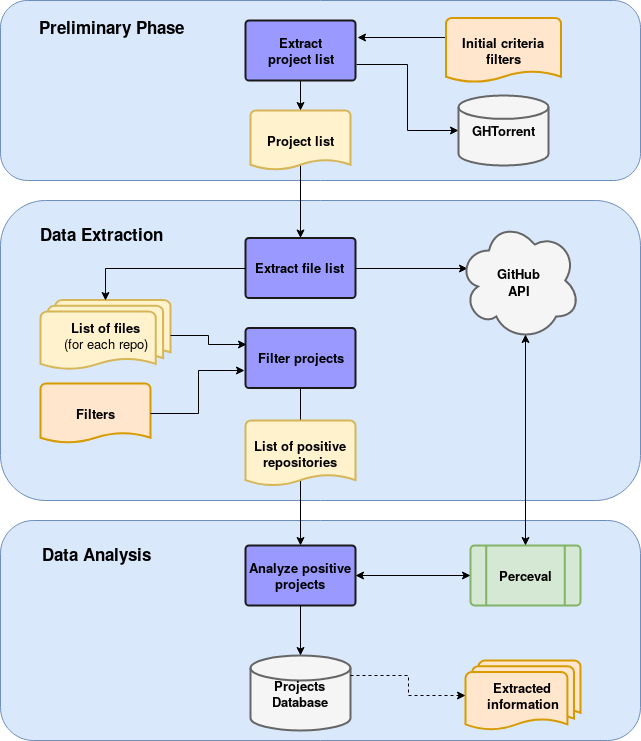
\includegraphics[width=15cm, keepaspectratio]{img/generic-tool-diagram-sections}
  \caption{General architecture of the tool}
  \label{fig:arquitectura}
\end{figure}
%%%%%%%%%%%%%%%%%%%%%%%%%%%%%%%%%%%
\section{Preliminary phase}
\label{sec:preliminary-phase}
Given the scale of GitHub, the main problem we face is that there isn't a direct way
of obtaining the amount of repositories in the platform, neither getting a list of them using its \textit{API}, so it is
very difficult to have quantitative and reliable data. For example, for building a graph like ~\ref{fig:total-repo-number},
its numbers had to be obtained directly from articles written by the GitHub team itself [\textcolor{red}{Source}]
and other people's estimations [\textcolor{red}{Source}].\par
At this point is where \emph{GHTorrent} project has its role in this story, as they provide an offline database dump with most
of the data which GitHub \textit{API} can provide at a certain date. This great collaborative effort is a huge advantage
for researchers, otherwise it would be practically non-viable retrieving full-scale GitHub data in a systematic way.
Nevertheless, it is important to mark that \emph{GHTorrent} database dump \underline{does not contain} \textit{Git trees}
(file-related) information: if this information was included, a major part of this tool (and by extension, this project) wouldn't
be necessary, as we could query and filter the data of our interest directly from the database which the \emph{GHTorrent} project provides.\\
If we have a look at how \emph{GHTorrent} database is structured (Figure~\ref{fig:ghtorrent-schema}), we can observe that
there is almost one table per GitHub object (\textit{users}, \textit{projects}, \textit{pull requests}, \textit{issues}, etc.).
Looking closer on these table's structure, we realize the table we need is the \emph{Projects} table
(see figure~\ref{fig:ghtorrent-schema-detail}), as it contains crucial repository-wise information including every project's name
and \textit{URL} but also other complementary information which could be used as a primary filter, like \texttt{language} (project's main language,
code-wise) or \texttt{forked\_from} (Empty if the repository isn't a \textit{fork} from another project), etc.\par
To obtain the actual data, the procedure to follow is:
\begin{enumerate}
  \item Download from \emph{GHTorrent} website a particular \emph{MySQL dump} which is provided as a compressed file in \texttt{tar.gz}
        format\footnote{To give an estimation of the current file sizes, the last dump available (2018, Mar 1st) sizes 71025 \texttt{MB}}.
  \item Uncompress the \texttt{tar.gz} file, which contains one \emph{CSV} file per table in the database.
  \item Get the file \texttt{projects.csv}, whose data corresponds to \emph{Projects} table (See an adapted\footnote{The field \emph{url} has been replaced by \emph{owner} to make the table more readable.}
  example of this file in table~\ref{table:projects-table-example}).
  \item Run the Python script \textcolor{red}{[reference to script]} with the corresponding filters to obtain the main
        \emph{project list} file, which will be the input for the next stage.
\end{enumerate}
Note that the filtering we establish in this phase is going to influence the results of our analysis. To make this task easier,
I decided to use a configuration file (See figure \textcolor{red}{[reference]}) to set basic filters and parameters. \textcolor{red}{(WIP)}\\
Finally, we obtain a filtered \emph{project list} file, which keeps the same format as \texttt{projects.csv} from the database dump.
\begin{figure}
  \centering
  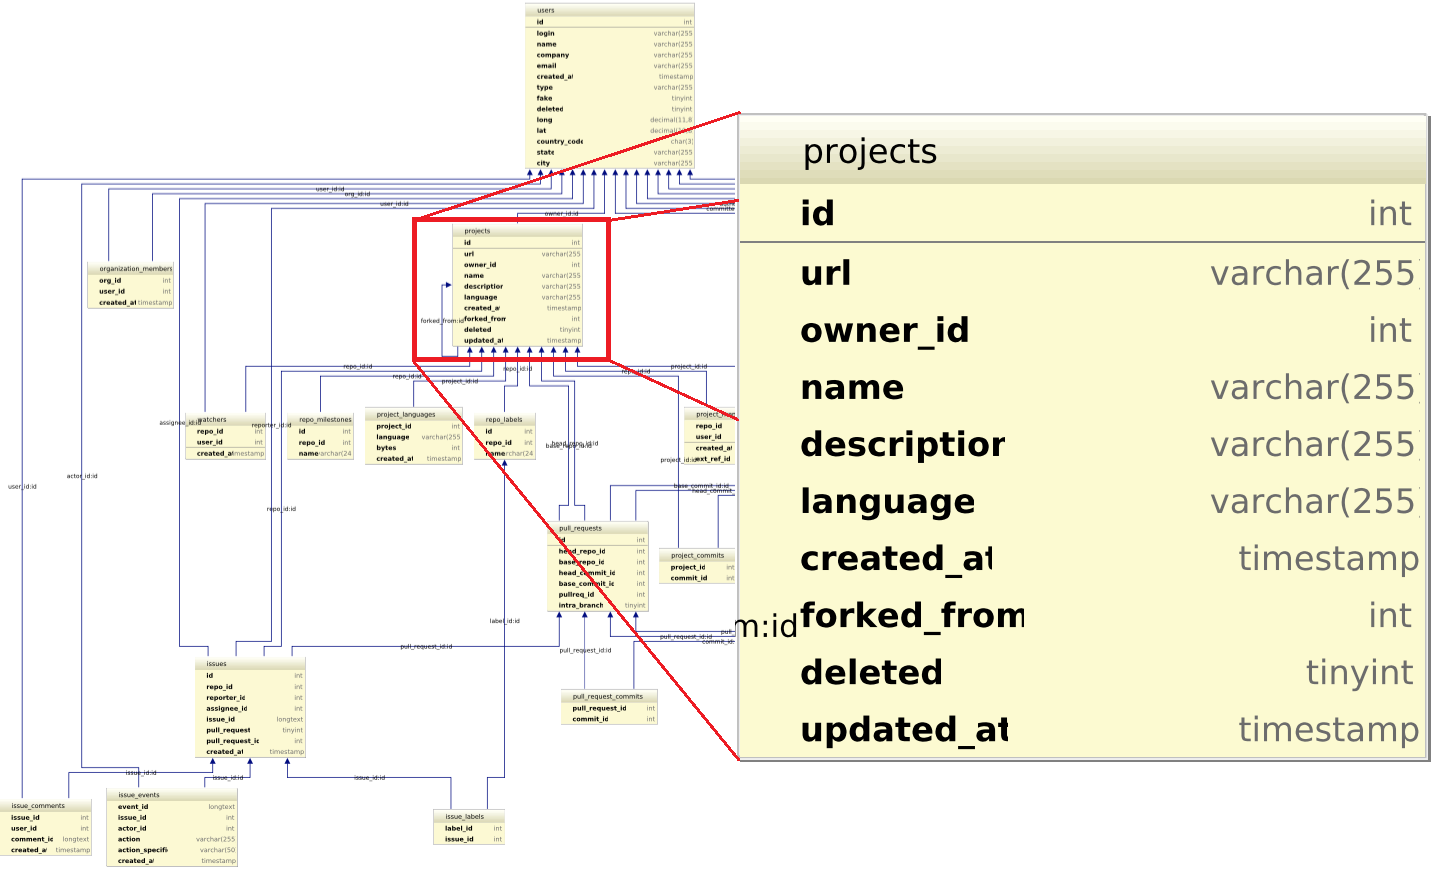
\includegraphics[width=16cm, keepaspectratio]{img/ghtorrent-schema-detail}
  \caption{\textit{Projects} table structure from GHTorrent database}
  \label{fig:ghtorrent-schema-detail}
\end{figure}
\begin{table}[]
\centering
\caption{Adapted extract from \texttt{projects.csv} file, formatted as a table}
\label{table:projects-table-example}
\resizebox{\textwidth}{!}{%
\begin{tabular}{|c|c|c|c|c|c|c|c|c|c|}
\hline
\textbf{id} & \textbf{owner} & \textbf{owner\_id} & \textbf{name} & \textbf{descriptor} & \textbf{language} & \textbf{created\_at} & \textbf{forked\_from} & \textbf{deleted} & \textbf{updated\_at} \\ \hline
20 & chrisjaure & 80 & git-lava & Branching metaphor for git & Shell & 2012-02-27 02:45:44 &  -  & 0 & 2015-10-18 01:39:38 \\ \hline
21 & ES-DOC & 82 & django-cim-forms & - & Python & 2012-03-23 14:20:28 &  -  & 1 & 0000-00-00 00:00:00 \\ \hline
23 & adammark & 86 & Markup.js & Powerful JavaScript templates & JavaScript & 2011-08-23 00:30:04 &  -  & 0 & 2015-10-12 10:46:04 \\ \hline
24 & leoamigood & 88 & 1stdibs\_V2.1 & Initial setup with mule-pull project & Java & 2012-05-03 11:43:31 &  -  & 1 & 0000-00-00 00:00:00 \\ \hline
\end{tabular}%
}
\end{table}
%%%%%%%%%%%%%%%%%%%%%%%%%%%%%%%%%%%
\section{Data extraction}
Once the \emph{project list} file is ready, we can proceed to extract the file list of the main \textit{branch} of each
repository. To achieve this, we have to query the GitHub \textit{API} several times for each project.
It is important to mark this, as the GitHub \textit{API} has a limitation of
5.000\footnote{The numbers (excepting dates) in this thesis follow the spanish separators notation.}
queries per hour for every authenticated account, which caused a huge impact in the research and the data-retrieval
process, as it is detailed in the case of study described in section~\ref{sec:case-study-uml}.\par
To make authenticated queries to the GitHub \textit{API} we need an \textbf{API token}\footnote{See the definition for API token in subsection~\ref{ssec:api-token}}.
For instance, if I want to \textit{fork} a repository into my GitHub account, I could do it either in two ways:
\begin{itemize}
  \item Log-in into my account, visit the repository \emph{URL} and press the \textbf{fork} button on GitHub's web interface.
  \item Send an authenticated \textit{query}\footnote{From now on, every time I refer to a GitHub \textit{API}
  request I will omit \texttt{https://api.github.com}.}
  to the GitHub \textit{API} like this one\footnote{On the requests, the parameters are marked with two dots (:).}:
  \begin{lstlisting}[language=bash]
  POST https://api.github.com/repos/:owner/:repo/forks?:token \end{lstlisting}
\end{itemize}
The script for this phase, \texttt{github-api.py} (See its diagram in figure~\ref{fig:gh-api-diagram}) has into account
this API limitation, ensuring that this limit is not exceeded. It employs three different directories in order to classify its outputs:
\textbf{master}, \textbf{default} and \textbf{trees}.
Then, it reads the \emph{project list} file and, per line, executes the following actions:
\begin{itemize}
  \item Check if the repository corresponding to that line has been downloaded before by looking at the existing files
  in the directories \textbf{master} or \textbf{default}.
  \item If not, try to obtain data from the \emph{master} \textit{branch}, whose output will be saved into the directory
  \textbf{master}.
  The \textit{query} sent to the GitHub \textit{API} to retrieve this data is:
  \begin{lstlisting}[language=bash]
  GET /repos/:owner/:repo/branches/master?:token \end{lstlisting}
  If we obtain a successful response, we will have a \texttt{JSON} file similar to the one in figure~\ref{fig:gh-api-master-json}.
  \item If the \emph{master} \textit{branch} is not found, we have to obtain the default \textit{branch} for that repository and
  perform another \textit{query} to retrieve the data from that \textit{branch}, which will be saved into the directory \textbf{default}.
  To retrieve this information, we need to obtain meta-data from the repository first and then, keep the content
  of the variable \texttt{default\_branch} to perform another \textit{query} to obtain data from that \textit{branch}:
  \begin{lstlisting}[language=bash]
  GET /repos/:owner/:repo?:token
  GET /repos/:owner/:repo/branches/:default_branch?:token \end{lstlisting}
  \item The last step is to read the obtained \texttt{JSON} data and get the tree objects recursively using the ID
  (\textit{SHA hash}) of the first one found in the response:
  \begin{lstlisting}[language=bash]
  GET /repos/:owner/:repo/git/trees/:sha?recursive=1&:token \end{lstlisting}
  This will be saved into the directory \textbf{trees}.
\end{itemize}
When this script finishes, we will have (assuming there were no errors) one \texttt{JSON} file per repository,
with the file-list information for the \textit{tree} objects in each repository.\\
However, the design of this script wouldn't be complete without considering all the possible errors and
particularities that may appear. Below, it is shown the most relevant setbacks and, if possible, an alternative
solution for every one of them:
\begin{itemize}
  \item \textbf{Private repository}. Some repositories in GitHub can be private if their owner hires a special
  plan on GitHub. The only solution is to perform the request with
  a token with granted access permissions to that repository, otherwise private repositories are ignored.
  \item \textbf{Truncated response}. Some repositories are too large so their tree and blob information is not completely
  sent within the response, but only a part of it and a Boolean field called \texttt{truncated} set to \texttt{True}.
  This was something that the GitHub \textit{API} implemented while we were performing the data retrieval of our
  use case, so we had to adapt the tool for it. The solution is to \textit{clone} (download) the repository,
  so later the next script can iterate locally over its files and folders.
  \item \textbf{Repository no longer exists}. There are repositories which existed at the time when that particular
  dump of the GHTorrent database was created, but they don't exist anymore.
  \item \textbf{\textit{Charset}-related errors}. Either the name of the repositories, owners, files, etc. can be written
  using different types of characters (Japanese, for instance) or other unknown characters (using another encoding)
  which sometimes caused encoding-decoding errors.
\end{itemize}
\label{sec:data-extraction}
\begin{figure}
  \centering
  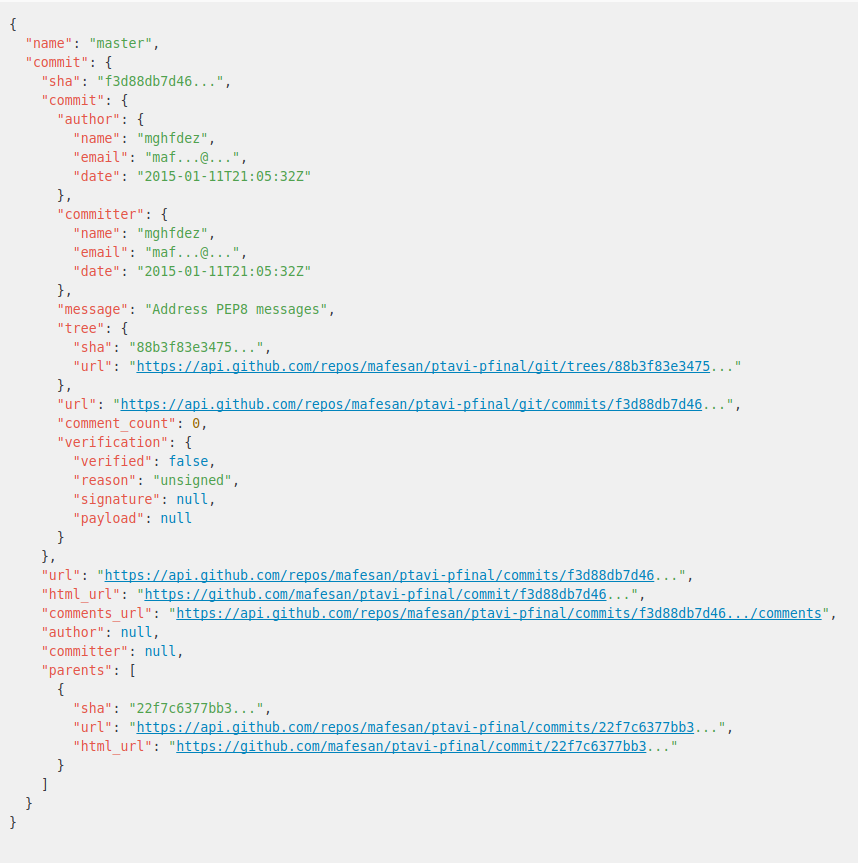
\includegraphics[width=13cm, keepaspectratio]{img/gh-api-master-json-example}
  \caption{Example: \texttt{JSON} response to the query asking for master branch data}
  \label{fig:gh-api-master-json}
\end{figure}
\begin{figure}
  \centering
  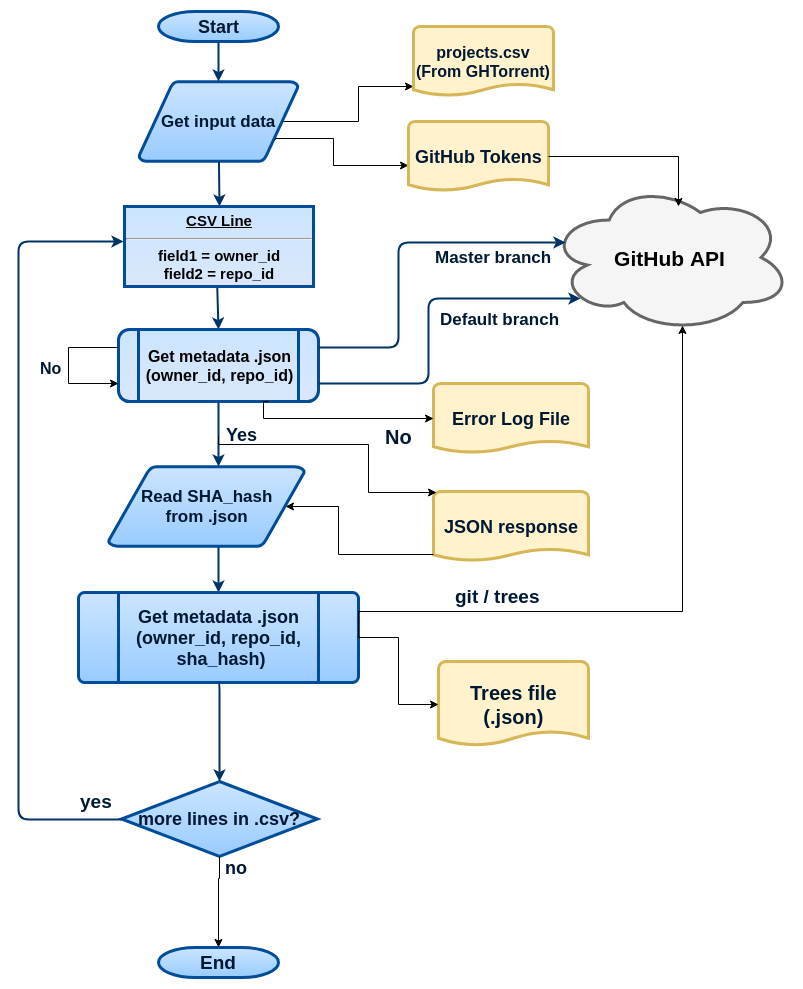
\includegraphics[width=14cm, keepaspectratio]{img/github-api}
  \caption{Flow-chart of \texttt{github-api.py} script}
  \label{fig:gh-api-diagram}
\end{figure}
%%%%%%%%%%%%%%%%%%%%%%%%%%%%%%%%%%%
\section{Data filtering}
\label{sec:data-filtering}
In this section is where the data we have obtained from the previous stage is filtered according to our search.
The approach that have been followed to apply filters is to define three types of heuristics, related to
file extensions and keywords:
\begin{itemize}
  \item \textbf{Level-1} file extensions, those which are a top priority in our search. They are immediately considered
   as positive results.
  \item \textbf{Level-2} file extensions, marked as relevant only if they meet one or more additional conditions.
  \item \textbf{Key-words}, specific words or groups of characters which a file-name with a \textit{Level-2} extension
  has to contain to be considered as a positive result.
\end{itemize}
Let's imagine a basic example where we are interested in projects related with web development. Defining the
necessary heuristics as in table~\ref{table:heuristics-table-example}, we will keep any file whose extension
is on Level-1 list, and those files whose extension is on Level-2 list \textbf{AND} whose file-name contains at least one
of the words (or group of characters) defined in the key-word list.\\
\begin{itemize}
  \item \texttt{.html} is on \textbf{Level-1} list, so any file with \texttt{html} extension will be a positive result directly.
  \item \texttt{.py} is on \textbf{Level-2} list, so only \texttt{.py} files containing at least one key-word in their file-name
  (i.e. \textit{urls}) will be considered as a positive result.
\end{itemize}
To complete this example, if we apply this filter to a repository whose file structure is like the one in figure~\ref{fig:file-structure-example},
we would obtain the set of positive results showed at table~\ref{table:heuristics-positive-example}.\par
Now, the next step is applying these filters to the \texttt{JSON} files which have been obtained before.
Specifically, we are interested only in those files included into the \textbf{trees} directory.
Each of those files contains the file structure of the last version of its repository,
where the \textit{tree} object contains under itself all the files (\textit{blob} objects) and sub-directories
(other \textit{tree} objects). Every object, no matter if it is a \textit{tree} or a \textit{blob}, contains the following parameters:
\begin{itemize}
  \item \textbf{path}: Absolute path of that file or folder inside the repository.
  \item \textbf{mode}: This number shows file mode information (file type, permissions, etc.) using UNIX notations.
  \item \textbf{type}: This value will be \texttt{blob} if it is a file, or \texttt{tree} if it is a folder.
  \item \textbf{sha}: Unique identifier for that \emph{git} object.
  \item \textbf{size}: File size in \textit{bytes}. Only \texttt{blob} objects contain this parameter.
  \item \textbf{url}: Link to this object in GitHub \textit{API}.
\end{itemize}
There is a simple example of the content of one of these files at figure~\ref{fig:gh-tree-json}.\par
The corresponding scripts for this phase are \texttt{github-tree.py} and \texttt{hits2urls.py}
(See a diagram for both of them in figure~\ref{fig:gh-tree-diagram}):\\
\texttt{github-tree.py} iterates over all the \texttt{JSON} files in the \textbf{trees} directory,
executing these simple instructions per file:
\begin{itemize}
  \item Load \texttt{JSON} data into a \emph{Python} \textit{dictionary} (a key-value data structure).
  \item Obtain the parent \texttt{tree} object (field \texttt{"tree"} in our \textit{dictionary}).
  \item Check the \texttt{"type"} field for every child object.
  \item If its type is \texttt{"blob"}, apply the pre-defined patterns and heuristics.
  \item Provide the positive results printing every matching object's \texttt{"path"} and \texttt{"URL"}.
\end{itemize}
\texttt{hits2urls.py} is a simple script which converts every \texttt{URL} from the last script (links to \texttt{blob} objects
in the GitHub \textit{API}), to the \texttt{URL} for the actual file which that object is representing to.
Here is an example of one \texttt{URL} which belongs to a \texttt{blob} object converted to the \texttt{URL}
pointing to the actual file (see below lines 1 and 2, respectively):
\begin{lstlisting}[language=bash]
https://api.github.com/repos/mafesan/ptavi-pfinal/git/blobs/3eb76189a21a...
https://raw.githubusercontent.com/mafesan/ptavi-pfinal/master/uaclient.py \end{lstlisting}
\begin{figure}
  \centering
  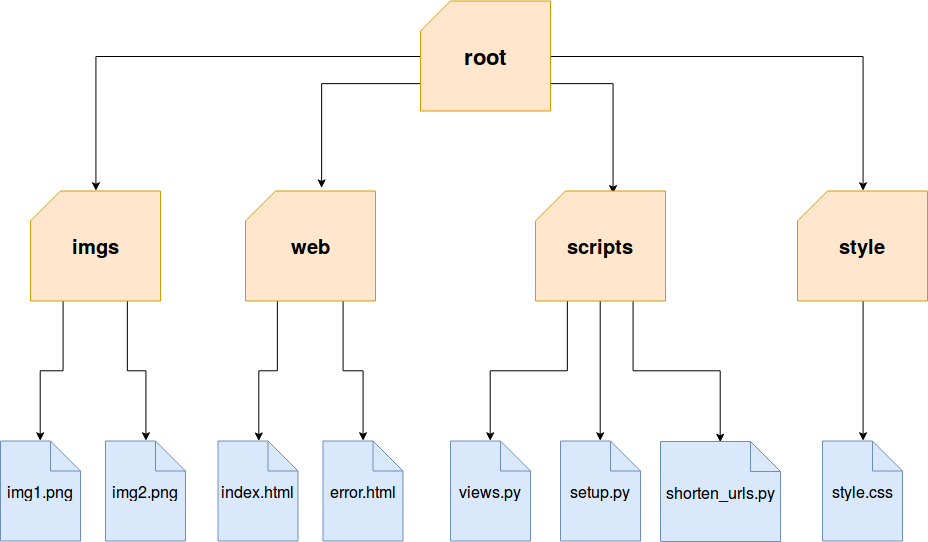
\includegraphics[width=13cm, keepaspectratio]{img/file-structure-example}
  \caption{Example: File-structure of a project to apply filters.}
  \label{fig:file-structure-example}
\end{figure}
\begin{figure}
  \centering
  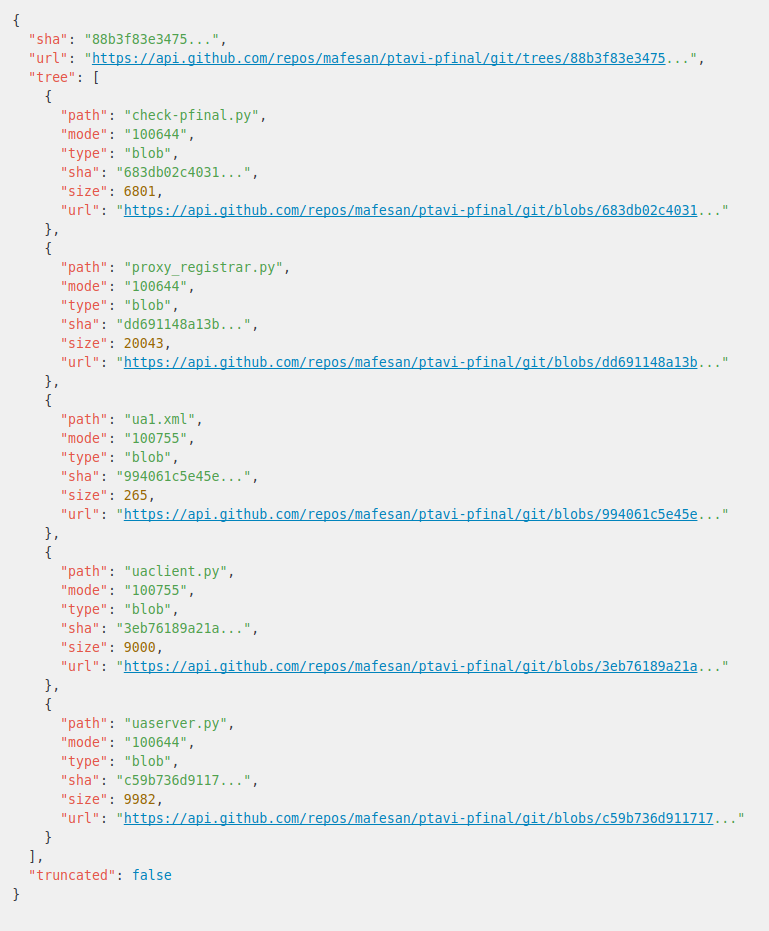
\includegraphics[width=13cm, keepaspectratio]{img/gh-api-trees-json-example}
  \caption{Example: \texttt{JSON} file containing information about \textit{tree} objects}
  \label{fig:gh-tree-json}
\end{figure}
\begin{figure}
  \centering
  \includegraphics[width=11cm, keepaspectratio]{img/github-tree}
  \caption{Flow-chart with the functioning of \texttt{github-tree.py} and \texttt{hits2urls.py} scripts.}
  \label{fig:gh-tree-diagram}
\end{figure}
\begin{table}[]
\centering
\caption{Example: definition of heuristics.}
\label{table:heuristics-table-example}
\begin{tabular}{|c|c|}
\hline
\textbf{Type of Heuristic} & \textbf{Pattern(s)}                                            \\ \hline
Level-1                    & \textit{.html}, \textit{.css}, \textit{.js}                    \\ \hline
Level-2                    & \textit{.py}                                                   \\ \hline
Key-words                  & \textit{urls}, \textit{views}, \textit{forms}, \textit{models} \\ \hline
\end{tabular}
\end{table}
\begin{table}[]
\centering
\caption{Positive results after applying heuristics filter.}
\label{table:heuristics-positive-example}
\begin{tabular}{|c|c|}
\hline
\textbf{Path}              & \textbf{Type of positive}   \\ \hline
scripts/shorten\_urls.py & Level-2 + contains key-word   \\
scripts/views.py           & Level-2 + contains key-word \\
style/template.css         & Level-1                     \\
web/error.html             & Level-1                     \\
web/index.html             & Level-1                     \\ \hline
\end{tabular}
\end{table}
%%%%%%%%%%%%%%%%%%%%%%%%%%%%%%%%%%%
\section{Data analysis}
\label{sec:data-analysis}
In this section is where the positive results are analyzed deeply to end up building a database to store
all the extracted information so it can be queried to perform our desired analysis.
\subsection{Extract extended repository information}
\label{ssec:extract-perceval}
To analyze the resulting repositories we take advantage of \textbf{Perceval}, a mature, powerful tool which
is capable of retrieving data from more than 25 different data sources producing a uniform set of data which can be
updated along time.\\
The data sources which Perceval supports are given by its \emph{backends}, and we are using the \emph{Git backend} to
obtain Git-related information from those GitHub repositories with at least one positive result.
Perceval clones repository by repository and parses every Git event log, producing a \emph{JSON} file
per repository containing data for every commit and its related Git objects. This tool is written in Python
language and it can be executed via command line or as a Python module, so it can be easily integrated with
this set of scripts.\\
\subsection{Building the database}
\label{ssec:build-database}
Next step is to build a database, which allows to store the extracted data in an optimized way to
obtain elaborated results by using queries according to our case of study.\\
As we had used the GHTorrent database, which is a MySQL database, we decided to use a MySQL database
for this purpose too, as it is easier to build and maintain.
We designed this database to contain five tables; four of them using data from the files which are obtained with
\textbf{Perceval} and one table from the GHTorrent database, \texttt{USERS} containing information about GitHub user accounts.
These tables contain the following information:
\begin{itemize}
  \item \texttt{REPOS}: For a repository; its name, number of commits, URL, founder, etc.
  \item \texttt{PEOPLE}: Referring to the people who authored the commits, their name and email.
  \item \texttt{COMMITS}: For each commit object; its ID in Git, its ID on GitHub, which repository belongs to, ID of its author, etc.
  \item \texttt{INTERESTING\_FILES}: For each file (positive result); its name, URL, which repository belongs to and which commits this file is included into.
  \item \texttt{USERS}: From GHTorrent, GitHub user account information as login, name, location, company, creation date, etc.
\end{itemize}
After a first version of this database, it was decided to add an additional table, \textit{FILE\_COMMITS},
which contains augmented information about each file commit, indicating the commit unique ID, the name of the committed file and the field
file-type (type of the committed file based on a predefined classification, i.e., source code, documentation, etc.).
These tables are represented in the complete schema of this database in figure~\ref{fig:dbschema}.\par
The dedicated script which converts the analysed data into a database produces one SQL script per table. Then, these
scripts have to be imported in a MySQL database whose structure has to be specified before.
Once the database has been built and filled with the data, to produce proper results for our analysis we have to ensure
that the perform the right queries. For instance, here are some queries we can execute to perform an analysis:
\begin{itemize}
    \item Name of positive repositories with more than 200 commits and whose last commit has been made after July 2, 2017:
    \begin{lstlisting}[language=SQL]
    SELECT name FROM repos
    WHERE number_commits > 200
    AND last_commit >= "2017-07-02"; \end{lstlisting}
    \item Number of repositories with at least one file with \textit{.png} extension:
    \begin{lstlisting}[language=SQL]
    SELECT COUNT(DISTINCT repos.name) FROM interesting_files
    LEFT JOIN repos ON interesting_files.repo_id = repos.id
    WHERE interesting_files.name LIKE '\%.png'; \end{lstlisting}
\end{itemize}

\begin{figure}
  \centering
  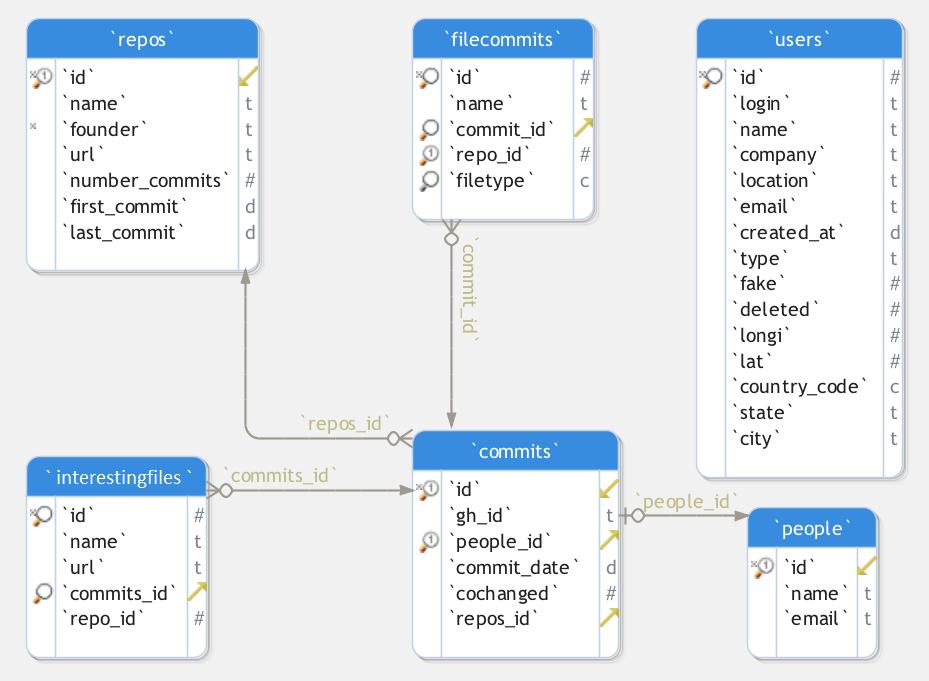
\includegraphics[width=15cm, keepaspectratio]{img/dbschema-generic}
  \caption{Database schema from the data-analisis phase.}
  \label{fig:dbschema}
\end{figure}
%%%%%%%%%%%%%%%%%%%%%%%%%%%%%%%%%%%%%%%%%%%%%%%%%%%%%%%%%%%%%%%%%%%%%%%%%%%%%%%%
%%%%%%%%%%%%%%%%%%%%%%%%%%%%%%%%%%%%%%%%%%%%%%%%%%%%%%%%%%%%%%%%%%%%%%%%%%%%%%%%
% RESULTADOS %
%%%%%%%%%%%%%%%%%%%%%%%%%%%%%%%%%%%%%%%%%%%%%%%%%%%%%%%%%%%%%%%%%%%%%%%%%%%%%%%%
\cleardoublepage
\chapter{Results}
\label{sec:results}
As I mentioned in section~\ref{sec:intro}, this project was born in a research environment.
In this current section it is described how the tool behaved in a real environment with all the setbacks
and limitations that appeared during the whole process, remarking that this ongoing research
influenced most of the decisions which were took during the design and implementation
of the tool that we saw in the last section, as well as how to overcome the different drawbacks.\par
The results presented here led to several scientific papers published on international Software Engineering
conferences which are highly ranked according to CORE\footnote{\url{http://www.core.edu.au/conference-portal}} portal:
\begin{itemize}
    \item ICSE (International Conference on Software Engineering) - Rank A* (Source\footnote{\url{http://portal.core.edu.au/conf-ranks/1209/}}).
    \item MODELS (International Conference on the Unified Modelling Language) - Rank A (Source\footnote{\url{http://portal.core.edu.au/conf-ranks/1244/}}).
    \item MSR (International Conference on Mining Software Repositories) - Rank A, before rank C (Source\footnote{\url{http://portal.core.edu.au/conf-ranks/711/}}).
\end{itemize}
The complete published papers are available in appendix~\ref{app:papers}.
\\This case of study descriptions are focused on the implementation of the technical part of the studies,
showing an overview of its results taking into account specific details and limitations.
%%%%%%%%%%%%%%%%%%%%%%%%%%%%%%%%%%%
\section{Case of study: UML models in GitHub projects}
\label{sec:case-study-uml}
This methodology was applied for the first time to the study: ”The quest for Open Source projects that use
UML: Mining GitHub” [HQC + 16 - cite] (The full paper is available in section~\ref{sec:paper-models}).
This research has been a collaborative work between Chalmers University and Rey Juan Carlos University in the context
explained in section~\ref{sec:context}.
The main goal of this study was to deepen in the knowledge of usage and evolution of UML models in
Free/Libre/Open Source Software (FLOSS) projects, tracking them throughout the whole projects life-span.
In addition to the main research questions mentioned in section~\ref{sec:objectives}, some of the specific RQs
of this study were:
\begin{itemize}
  \item RQ1: Are there GitHub projects that use UML? Which are these projects?
  \item RQ2: Are there GitHub projects in which the UML models are also updated?
  \item RQ3: When in the project are new UML models introduced?
  \item RQ4: What is the time span of ``active'' UML creation and modification?
\end{itemize}
It is important to know if there is some peculiarity in the data we are looking for, for example, UML models can be
found in many different formats, but they can be classified into two main types: text-based models, which are XML-alike
files and image-based models (See figure~\ref{fig:uml-types}). This entails an additional problem as an external validation of the data is
required in an intermediate step between the data filtering phase and the analysis one, which will be detailed later.\par
The first two phases of the tool, described in sections~\ref{sec:preliminary-phase} and~\ref{sec:data-extraction} respectively
are, by default, independent from the case of study. However, these phases are not a trivial task because of the amount of
data that has to be processed with the difficulties and limitations associated with it.\\
Regarding to the preliminary phase, the GHTorrent data-set used in this study is from February, 2016. At that time, there were
a total of 26 million repositories (approx.). As the main research that motivated this study was interested in identify UML
models introduced in a project by its owners, we had to filter those projects to discard forked repositories. Applying that
filter we got 12.847.555 repositories ready to be analyzed.\par
The greatest challenge was to execute the tool against almost 13 million GitHub repositories, as the GitHub API has a limitation
of 5.000 requests per hour \& account. As it is explained before, a maximum of three requests are made to obtain the main
branch for each repository, as we are not interested in secondary branches for our case of study. Making the calculations about
how much time would it take to complete this first stage:
\begin{itemize}
  \item 3 queries for each project = 1.666 projects/hour (max).
  \item 12.847.555 projects / 1.666 projects per hour = 7.712 h. = 322 days
\end{itemize}
We made an estimation where 322 days would be needed with the best scenario, so we opted for paralleling the process using many
different GitHub accounts.\\
To make this possible, we asked for help to some students and professors so they can temporarily borrow their GitHub account
token and we obtained 21 account tokens. Finally, it took almost 90 days to complete this task as we were receiving these credentials
while we were already collecting data. I take this opportunity to thank every person who had the kindness to contribute to this project
with their GitHub accounts.
In addition to the GitHub API limitation, we may encounter technical limitations: it is desirable to have a fast and stable Internet
connection, enough space in the hard drive and also use a powerful computer, as after the data-extraction stage we got 126 GB of compressed
JSON files, which have to be opened and processed.\par
To continue with the next step of the data extraction phase, which is to apply the filter to the file-list information
we had obtained. In this case, we are interested in looking for files whose extension matches with all possible extensions which an
UML model can be found, as is it showed in table~\ref{table:heuristics-cs1-example}.\par
As described before, an additional problem arose: from all the identified files with the interesting extensions, how many of those files
really are a UML model, and how many are not? As the tool has a modular design, it was easy to add an additional phase to verify the data
which was obtained after the filtering. This verification process was solved by Chalmers team, using heuristics for the XML-alike files
and image processing and machine learning techniques for image files [HQCS + 14a, HQCS + 14b - \textcolor{red}{FIXME: Citations}].\par
UML models can be included either in image or text files (See figure~\ref{fig:uml-types}), therefore our main filter using file extensions
and character patters in file-names is not enough to completely identify UML files. That is why it was necessary the inclusion of
an additional phase where all the positive outcomes after applying the first filter (now marked as \textbf{potential files}) need
to be validated to determine whether they contain a UML model or not. This external validation stage developed by \emph{Chalmers} team
includes machine-learning and digital image processing techniques which also required manual verification steps, which were very time-consuming.\\
This handicap led to the decision of shorten the data-set to analyze $\sim$10\% of the total amount of GitHub repositories which resulted
in 1.240.000 repositories, in order to offer accurately verified results. From those repositories, we obtained 100.702 potential files
which matched after applying the heuristics filter in table~\ref{table:heuristics-cs1-example}. These potential files are the input
of the validation stage whose process and results are summarized on figure~\ref{fig:validated-files-distribution}: A total of 21.316 UML
files were validated included in 3.295 different GitHub repositories, which is the answer to RQ1.\par
Next, in the data-analysis phase these projects were processed with Perceval and a database was built using that information.
Once the database was created it was obtained more elaborated data, for instance, the distribution of positive repositories
according to how many UML models contained each of them (See table~\ref{table:validated-repos-table}) but also the answers to the rest
of the RQs:
\begin{itemize}
  \item RQ2: Are there GitHub projects in which the UML models are also updated?
  \begin{itemize}
    \item Only 26\% of this first data-set updated their UML files at least once.
  \end{itemize}
  \item RQ3: When in the project are new UML models introduced?
  \begin{itemize}
    \item UML models are introduced in all active phases of a project with a tendency towards the early phases.
  \end{itemize}
  \item RQ4: What is the time span of ``active'' UML creation and modification?
  \begin{itemize}
    \item Few of the studied projects are active with UML during their whole lifetime.
    In general, the projects work very shortly in UML, usually at the beginning.
  \end{itemize}
\end{itemize}
hen the validation process described before was extended to the whole set of potential results, the UML search was finished.
These complete results were presented in the paper "An extensive dataset of UML models in GitHub" (The full paper is available in section~\ref{sec:paper-msr}),
which resulted in the identification of 93.596 (See table~\ref{table:validated-models-table} publicly available UML models
in GitHub from over 24.125 repositories. Though this amount of repositories only represent 0,19239\% of the total amount of the initial set,
as I anticipated in the introduction chapter, the identified models constitute a data-set that is two orders of magnitude larger than the
rest of UML data-sets at the time of this research.\par
Applying the data-analysis phase to the complete UML models data-set we ended up with a database with deeper information about these results,
which broaden the possibilities to enrich different aspects of this research. This derived in the paper "Practices and Perceptions of UML Use
in Open Source Projects" (The full paper is available in section~\ref{sec:paper-icse}), whose goal of this later research was ``to shed some
light into the motivation and benefits of the use of modeling and its use within project teams''. To do so, the applied method was to
perform a survey among open source developers, focusing on projects that use UML as a representative for software modeling.\\
The constructed database played a pivotal role for this survey, as it was necessary to define which projects and developers met the
survey conditions executing the right queries to the database. There were two main lines to obtain the survey target:
\begin{enumerate}
  \item \textbf{Filtering short-time projects out}: For this paper, researchers aimed
  at projects that are interesting from an industry perspective. Then, we focus on projects that are \textbf{not} short-term and that
  do not jut consist of a singe contributor. In this context, the accurate definitions of ``short-time project'' are:
  \begin{enumerate}[i.]
    \item Active time (time between the first and the latest commits) less then 6 months, OR
    \item less than 2 contributors, OR
    \item less than 10 commits.
  \end{enumerate}
  After classifying and filtering short-time projects out, 4.650 UML-projects (out of 24.125) met the requirements.
  \item \textbf{Identify developer role in a repository}: It was important to consider the role that the different contributors
  play within the OSS projects with UML models to ask them the appropriate questions, considering a combination of roles in the
  following two dimensions:
  \begin{enumerate}[i.]
    \item Founder (F) vs. non-founder (NF)
    \item Non-UML Contributor (NUC) vs. first UML Contributor (1UC) \& UML Contributor or updater (non-1st contributor) (UC)
  \end{enumerate}
  Therefore, each interview participant had to fulfill one of the following 6 roles: F-1UC, F-NUC, F-UC, NF-1UC, NF-NUC, NF-UC.
\end{enumerate}
Furthermore, researchers considered the possibility of having duplicate identities in our database, as one contributor can
use different emails, user-name (for example, changing the user-name or email during the project time).
The email and the full-name were the primary keys for this check, which resulted in 99.319 distinct contributors out of
129.276 original ones.
 \begin{figure}
   \centering
   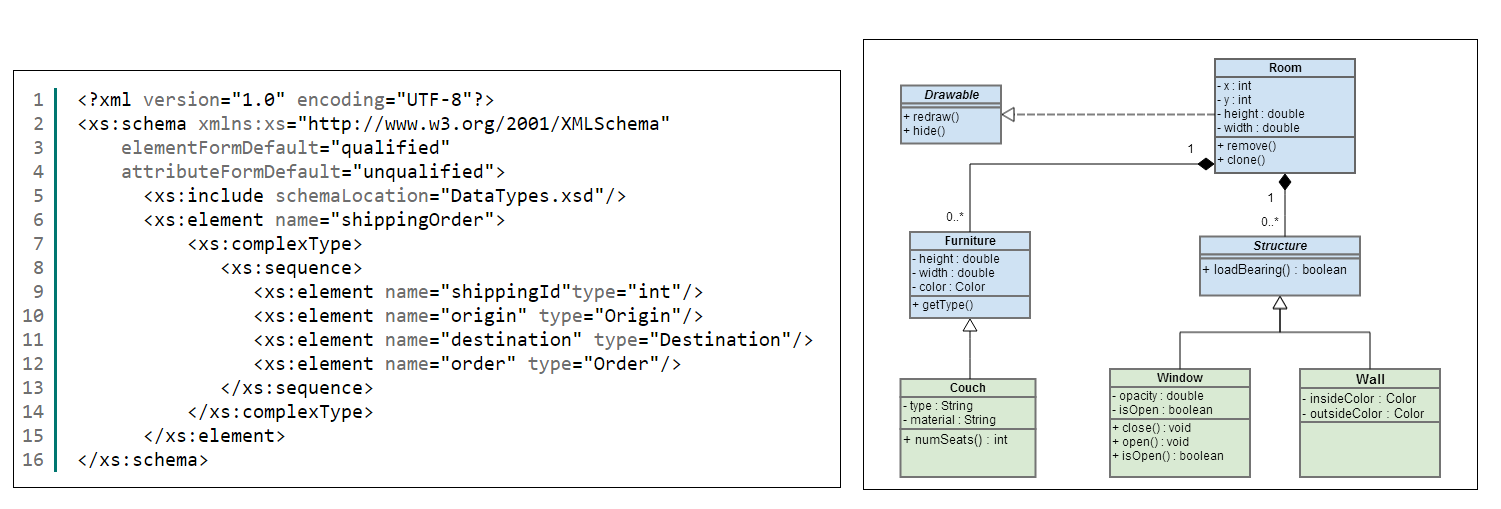
\includegraphics[width=15cm, keepaspectratio]{img/umls-landscape}
   \caption{Examples of how UML models can be found, text-based (left) or image type (right).}
   \label{fig:uml-types}
 \end{figure}
 \begin{table}[]
 \centering
 \caption{Example: definition of heuristics for the case of study 1.}
 \label{table:heuristics-cs1-example}
 \begin{tabular}{|c|c|}
 \hline
 \textbf{Type of Heuristic} & \textbf{Pattern(s)}                                                                                           \\ \hline
 Level-1                    & \textit{.uml}, \textit{.xmi}, \textit{.uxf} and \textit{.xdr}                                                 \\ \hline
 Level-2                    & \textit{.xml}, \textit{.bmp}, \textit{.jpg}, \textit{.jpeg}, \textit{.gif}, \textit{.png} and \textit{.svg}   \\ \hline
 Key-words                  & \textit{xmi}, \textit{uml}, \textit{diagram}, \textit{architecture} and \textit{design}                       \\ \hline
 \end{tabular}
 \end{table}
 \begin{figure}
   \centering
   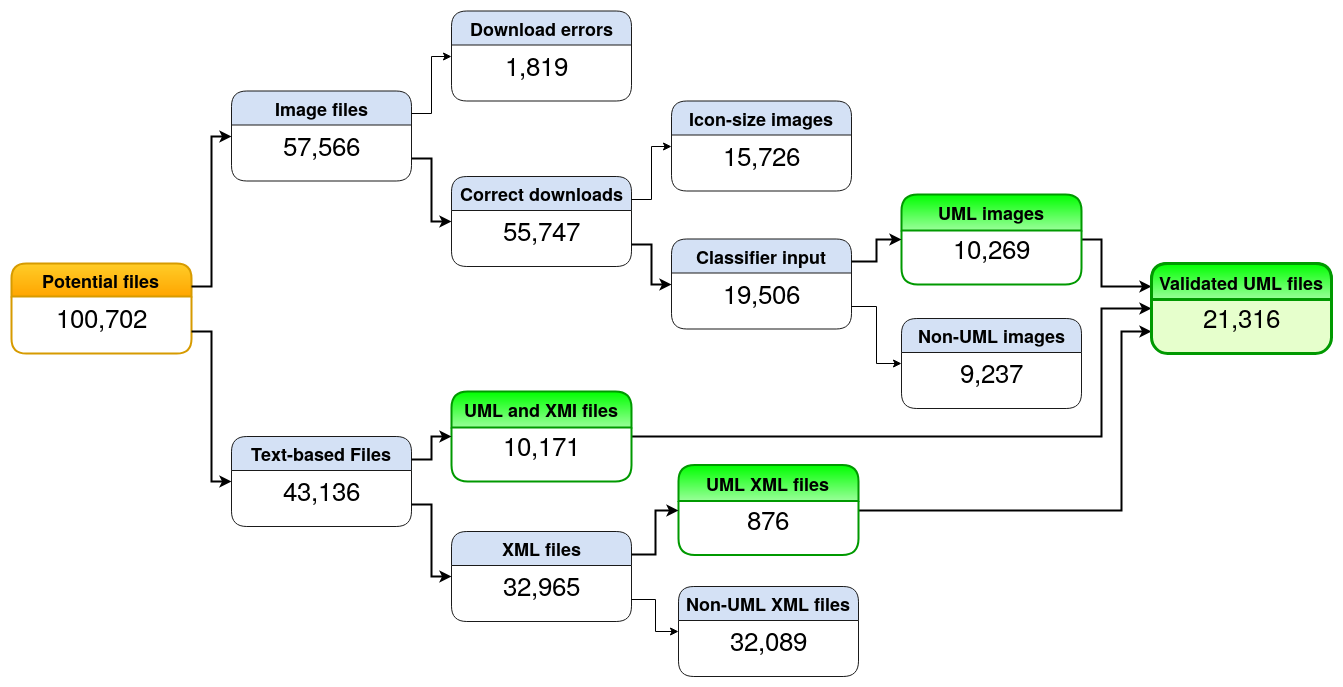
\includegraphics[width=16cm, keepaspectratio]{img/file-results-models-diagram}
   \caption{Diagram: Results distribution from potential files to validated UML files.}
   \label{fig:validated-files-distribution}
 \end{figure}
 \begin{table}[]
   \centering
   \caption{Validated positive repositories (partial) sorted by their number of UML models.}
   \label{table:validated-repos-table}
   \begin{tabular}{|c|c|}
   \hline
   \textbf{Number of UML models} & \textbf{Number of repositories}     \\ \hline
   1                             & 1.947                               \\
   From 2 to 9                   & 1.169                               \\
   From 10 to 99                 & 158                                 \\
   100+                          & 4                                   \\ \hline
   \end{tabular}
 \end{table}
 \begin{table}[]
   \centering
   \caption{Complete results of validated positive UML models sorted by their type.}
   \label{table:validated-models-table}
   \begin{tabular}{|c|c|}
   \hline
   \textbf{Type of model}     & \textbf{Number of UML models}     \\ \hline
   Text-based (.uml, .xmi)    & 35.774                            \\
   Image-based                & 57.822                            \\ \hline
   \end{tabular}
 \end{table}
%%%%%%%%%%%%%%%%%%%%%%%%%%%%%%%%%%%%%%%%%
\section{Case of study: Software Architecture documents \& extended UML models in GitHub projects}
\label{sec:case-study-sad}
After the derived studies from the first data-set, the second case of study came out when the same research team were
interested in extend the search looking for models with other less-restrictive extensions but also looking for
software architecture documents, as sometimes the models from a project are defined inside a document (i.e., a PDF file).\\
Accomplishing this new case of study was substantially easier and faster, as all the JSON files containing file-related information
from all GitHub projects were already downloaded. Then, with the preliminary and data-extraction phases completed, the procedure to
follow was to execute the steps from the data-filtering stage using the patterns and heuristics from table~\ref{table:heuristics-cs2-example}.
This data-filtering phase resulted in a list of 6.373.748 potential files belonging to 573.854 different GitHub repositories.
Since these potential results haven't been validated yet, no further phases of the tool were executed.
\begin{table}[]
\centering
\caption{Example: definition of heuristics for the case of study 2.}
\label{table:heuristics-cs2-example}
\begin{tabular}{|c|c|}
\hline
\textbf{Type of Heuristic} & \textbf{Pattern(s)}                                                                                           \\ \hline
Level-1                    & \textit{.uml}, \textit{.xmi}, \textit{.uxf}, \textit{.xdr}, \textit{.eap}, \textit{.aird}, \textit{.argo},    \\
                           & \textit{.asta}, \textit{.dfClass}, \textit{dfUseCase}, \textit{.ecore}, \textit{.ecorediag}, \textit{.umlcd}, \\
                           & \textit{.mdj}, \textit{.plantuml}, \textit{.simp}, \textit{.txvcls}, \textit{.umlx}, \textit{.ump},           \\
                           & \textit{.uxf}, \textit{.zargo}, \textit{.zuml}, \textit{.zvpl}, \textit{.dia}, \textit{.modelproj},           \\
                           & \textit{.classdiagram}, \textit{.sequencediagram}, \textit{.activitydiagram}, \textit{.usecasediagram},       \\
                           & \textit{.componentdiagram}, \textit{.layerdiagram}, \textit{.cd}, \textit{.di} and \textit{.umldi}            \\ \hline
Level-2                    & \textit{``''}, \textit{.xml}, \textit{.bmp}, \textit{.jpg}, \textit{.jpeg}, \textit{.gif}, \textit{.png},     \\
                           & \textit{.svg}, \textit{.txt}, \textit{.doc}, \textit{.docx}, \textit{.ppt}, \textit{.pptx} and \textit{.pdf}  \\ \hline
Key-words                  & \textit{xmi}, \textit{uml}, \textit{diagram}, \textit{architecture}, \textit{design}, \textit{sad},           \\
                           & \textit{sdd}, \textit{arch} and  \textit{hier}                                                                \\ \hline
\end{tabular}
\end{table}
%%%%%%%%%%%%%%%%%%%%%%%%%%%%%%%%%%%%%%%%%%%%%%%%%%%%%%%%%%%%%%%%%%%%%%%%%%%%%%%%
%%%%%%%%%%%%%%%%%%%%%%%%%%%%%%%%%%%%%%%%%%%%%%%%%%%%%%%%%%%%%%%%%%%%%%%%%%%%%%%%
% CONCLUSIONES %
%%%%%%%%%%%%%%%%%%%%%%%%%%%%%%%%%%%%%%%%%%%%%%%%%%%%%%%%%%%%%%%%%%%%%%%%%%%%%%%%
\cleardoublepage
\chapter{Conclusions}
\label{sec:conclusions}
During the whole implementation and the later set-up process of this tool with the different use-cases,
there were found several handicaps, limitations and setbacks which affected how the objetives described
in chapter~\ref{sec:objectives} were reached. Nonetheless, looking back at the tool and how
it performed with the different use-cases, along with the obtained results, it is safe to
say the purpose of this tool was achieved, proving answers to the proposed research questions.
%%%%%%%%%%%%%%%%%%%%%%%%%%%%%%%%%%%
\section{Achieved objectives}
\label{sec:achieved-objectives}
Regarding OB1\footnote{Extract the whole set of projects hosted in GitHub.},
we were able to extract the whole set of projects hosted in GitHub at
a certain date and time thank to the \emph{GHTorrent} project. This is the first threat
following this approach: during the time where the MySQL dump of \emph{GHTorrent} from GitHub data is created
and the data extraction phase is executed, the source of information is constantly changing,
so we may encounter some projects that don't exist anymore, some projects become private
and of course, there are new projects that are being created. These limitations are hard
to avoid but also it is safer to extract the information from an static, reliable and uniform source.\par
About OB2\footnote{Collect data from all public projects about their file structure in a scalable, automated way.},
this was the most arduous objective to accomplish, as setting up and watching over
the different parallel instances (up to 21 instances running at the same time) to speed-up the completion
of the whole data-retrieval process required a huge amount of time and effort. The GitHub API limit of
5.000 requests per hour \& account was a huge drawback we tried to avoid contacting to GitHub asking them for a special
account without limitation in order to perform the study, but the solution they gave us was to create more accounts
and using them all to perform more requests per hour (and so we did). Furthermore, GitHub API changed during this
data-retrieval phase including paginated results. That forced us to adapt this tool and re-analyse some of the data
that have been already dowloaded.\\
These drawbacks could be avoided in future versions of this tool if \emph{GHTorrent} included git-trees information. It would save a lot of time and resources,
together with having more reliability due to the staticness this data would have.\par
Looking at OB3\footnote{Establish a procedure to filter this extracted data using a determined kind of heuristics and patterns.},
the positive results can be identified properly. However, due to the different particularities of the data
we want to analyse, we may want to add more filtering layers to the obtained potential results. Technically,
the most difficult issue was to handle huge JSON files (some of them sized GBs) and cover the diverse Charset-related
errors.\par
OB4\footnote{Analyze positive GitHub repositories to obtain enhanced Git data from them.}
was completely covered using \emph{Perceval}, with the limitations of encountering positive repositories which had been deleted
or set as private, reducing the final data-set.
Finally, OB5\footnote{Store the enhanced data in a database whose structure allows to query information of interest.}
was also completely accomplished. These two last objectives
share some technical difficulties regarding to storage space and performance: Perceval needed to clone the repositories,
which means it had to download and uncompress data; and some of the generated SQL files with the database information
(like the one for the \texttt{commits} table) contained millions of entries, which aside from their size, difficulted
the importing process.\par
%%%%%%%%%%%%%%%%%%%%%%%%%%%%%%%%%%%
\section{Knowledge application}
\label{sec:knowledge-application}
During my degree I've learned about important concepts and tools during the different courses,
but also about how to face new challenges where to implement the acquired knowledge.
In this project I have applied the learning outcomes from the following courses:
\begin{enumerate}
  \item \textbf{``Informática I''} (Fundamentals of Programming): This course was my first programming-related course,
  where I learned the basics of programming'' (basic data and flow-control structures).
  \item \textbf{``Informática II''} (Telecommunication Systems Programming): In this course I learned advance programming
  techniques along with more complex data structures, including for the first time communication protocols as UDP and TCP connections
  ellaborating both client-server and peer-to-peer applications.
  \item \textbf{``Arquitectura de Internet''} and \textbf{``Sistemas Telemáticos para Medios Audiovisuales''} (Computer Networks I and II):
  Thank to these courses I learned about both basic and complex communication protocols and how the Internet works,
  from TCP/IP protocol to HTTP connections, routing algorithms and protocols, etc.
  \item \textbf{``Protocolos de Transmisión de Audio y Video en Internet''} (Audio/video Transmission Protocols):
  In this course I learned how to program in Python language and the basic concepts for object-oriented programming, in
  addition to real-time communication protocols.
  \item \textbf{``Laboratorio de Tecnologías Audiovisuales en la Web''} (Web-based Technologies): Though this course is not directly
  related, I learned basic concepts about databases and I fostered my programming skils in Python building my first Django
  application.
\end{enumerate}
%%%%%%%%%%%%%%%%%%%%%%%%%%%%%%%%%%%
\section{Learning outcomes}
\label{sec:learning-outcomes}
These are some of the learning outcomes I have obained thank to this project:
\begin{enumerate}
  \item Fostering of my programming skills, especially in Python. Though I was familiar with
  this programming language in particular, I've learned about general, complex concepts of programming
  as parallelization and concurrency but also specific advanced Python concepts and structures:
  sets (unordered collections of non-duplicated values), list-comprehensions
  (a way to to create lists containing an expression followed by a for clause, then
  zero or more for or if clauses) and other Python \textit{idioms}.
  \item Learning new technologies, specially about databases and SQL language which
  complements my academic background. I've also learn how to interact with APIs for the first time.
  \item A great overview about research. Since I started to work as a researcher assistant,
  I was surprised about how little I know about research and its procedures about scientific papers,
  conferences. With this project I was able to learn from the very beginning the stages of the elaboration
  of a study to its final stages including th process for the paper to be published.
  \item A valuable perspective about team work and communication, having the possibility
  to collaborate with an international team from a different university.
  \item System administration. Taking care of the technical tasks about this project forced me
  to learn how to execute and watch over all the stages of this tool in different environments,
  incluing remote servers.
\end{enumerate}
%%%%%%%%%%%%%%%%%%%%%%%%%%%%%%%%%%%
\section{Future work}
\label{sec:future-work}
This tool and its execution process can be improved in several aspects. Regarding to the preliminary and data-extraction
stages, these are some of the features that could be implemented:
\begin{itemize}
    \item A method to keep updated the initial set of GitHub projects from new dumps from \emph{GHTorrent}.
    \item If \emph{GHTorrent} dumps format change, adapt the necessary scripts to ensure compatibility.
    \item A method to keep updated the JSON files containing the file-list information for
    each repository, and another to unify the format of that data in those repositories whose response was truncated.
    \item Multi-thread execution support to have different parallel instances of \texttt{github-api.py} script.
    \item Improve monitoring and exception management.
\end{itemize}
In the data-filtering and the data-analysis phases, the proposed improvements are:
\begin{itemize}
    \item Add more filter types or improve the existing ones.
    \item Improve the method to analyze the positive repositories using Perceval. There is a new \emph{GrimoireLab}
    tool called \textbf{Arthur}\footnote{\url{https://github.com/chaoss/grimoirelab-kingarthur}},
    which is a distributed job queue platform that schedules and executes Perceval using threads, error management and more.
    This new tool could be integrated in the data-analysis stage to set the repositories to be analyzed by Perceval
    in a more efficient way.
    \item Optimize how the analyzed data is imported into a new database even exploring other different database types.
\end{itemize}
%%%%%%%%%%%%%%%%%%%%%%%%%%%%%%%%%%%
\section{Personal assessment}
\label{sec:assessment}
I had the great luck to be in the right place at the right moment when I started this project.
Working on it has brough me a lot of great experiences and outcomes, which are
extensive to my periord working as a reseacher assistant in LibreSoft group where I met fantastic people.\par
I feel fulfilled after having participated in such an important research and see its resulting scientific papers
presented and published in important conferences. I've obtained more knowledge but also self-confidence to face large-scale
projects, to make presentations in front of an audience and also to foster my english level. Furthermore,
I had the opportunity of travelling to Gothenburg (Sweden) in June, 2016 to meet the team from Chalmers University
we were collaborating with. Afterwards, this cooperation provided me the chance to enroll myself to an
ERASMUS+ traineeship in that university during summer 2017.\par
%%%%%%%%%%%%%%%%%%%%%%%%%%%%%%%%%%%%%%%%%%%%%%%%%%%%%%%%%%%%%%%%%%%%%%%%%%%%%%%%
%%%%%%%%%%%%%%%%%%%%%%%%%%%%%%%%%%%%%%%%%%%%%%%%%%%%%%%%%%%%%%%%%%%%%%%%%%%%%%%%
% APPENDIX %
%%%%%%%%%%%%%%%%%%%%%%%%%%%%%%%%%%%%%%%%%%%%%%%%%%%%%%%%%%%%%%%%%%%%%%%%%%%%%%%%
\cleardoublepage
\appendix
%%%%%%%%%%%%%%%%%%%%%%%%%%%%%%%%%%%%%%%%%%%%%%%%%%%%%%%%%%%%%%%%%%%%%%%%%%%%%%%%
%%%%%%%%%%%%%%%%%%%%%%%%%%%%%%%%%%%%%%%%%%%%%%%%%%%%%%%%%%%%%%%%%%%%%%%%%%%%%%%%
% DEFINITIONS %
%%%%%%%%%%%%%%%%%%%%%%%%%%%%%%%%%%%%%%%%%%%%%%%%%%%%%%%%%%%%%%%%%%%%%%%%%%%%%%%%
\chapter{Definitions}
\label{app:definitions}
%%%%%%%%%%%%%%%%%%%%%%%%%%%%%%%%%%%
\section{Git objects definitions}
\label{sec:git-definitions}
\subsection{Commit}
\label{ssec:git-commit}
A \textbf{commit} is a \emph{git} object which contains a record of the changes made to the repository since last modified
version of itself (last commit object). In the example in figure~\ref{fig:info-git}, each \textbf{commit} would be each different
\textit{Version} (1, 2, 3...), meaning that there is a new version of the repository with every \textbf{commit}.
\subsection{Tree}
\label{ssec:git-tree}
A \emph{git} \textbf{tree} represents a directory and its structure (including file-names) in the repository, containing other possible
sub-directories as other child \textbf{tree} objects. However, these objects do not contain any information about the file contents:
that is stored in \textbf{blob} objects. In figure~\ref{fig:git-objs-example} there is an example of how \textbf{commits},
\textbf{trees} and \textbf{blobs} are connected with each other.
\subsection{Branch}
\label{ssec:git-branch}
A \emph{git} \textbf{branch} is a pointer to a certain \emph{commit} object. All new commits
created from this pointer will diverge from the previous commit-history of the repository in two distinct, independent paths.
Branching is a very common and useful practice, as it allows to isolate different versions of the same files and directories
(but also different) in the same repository, and later, those branches can be merged into any other branch (See in
figure~\ref{fig:git-branches-example} a simplified example about the structure of a repository with several branches).
\begin{figure}
  \centering
  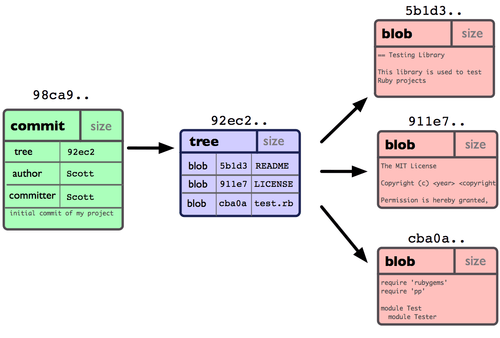
\includegraphics[width=12cm, keepaspectratio]{img/git-objs-example}
  \caption{Interaction among \textbf{commits}, \textbf{trees} and \textbf{blobs} (unique IDs above) (Source: Git documentation).}
  \label{fig:git-objs-example}
\end{figure}
\begin{figure}
  \centering
  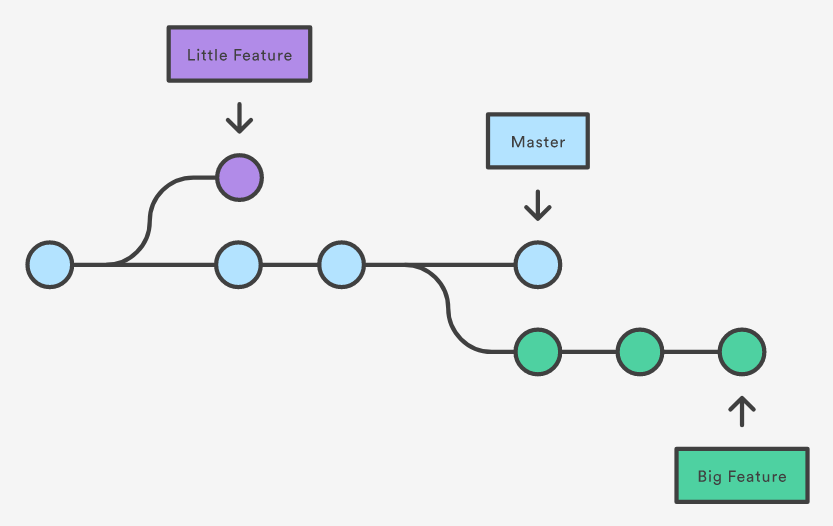
\includegraphics[width=12cm, keepaspectratio]{img/branches-example-atlassian}
  \caption{Abstraction of \emph{git} \textbf{branches} structure in a repository (Source: Atlassian).}
  \label{fig:git-branches-example}
\end{figure}
%%%%%%%%%%%%%%%%%%%%%%%%%%%%%%%%%%%
\section{API}
\label{sec:api}
An \textbf{API} (\textit{Application Programming Interface}) is a set of subroutine definitions, protocols, and tools for building
application software. In general terms, it is a set of clearly defined methods of communication between various software components.
\subsection{GitHub API}
\label{ssec:sec_gh-api}
GitHub \textit{API} allows to access GitHub data, since own GitHub types like \textit{pull-requests}, \textit{issues} or \textit{forks}
to \emph{git}-related data, such as \textit{commits}, \textit{branches} or \textit{trees} using \textit{HTTP} requests and
returning information using \emph{JSON} (\textit{JavaScript Object Notation}) format.
\subsection{API token}
\label{ssec:api-token}
A \textbf{token} is a unique identifier of an application requesting access to a service.
In the case of GitHub API, they are long, alphanumeric strings of characters generated within a GitHub account,
so every executed action with that \textbf{token} is done on behalf of its owner's account.
%%%%%%%%%%%%%%%%%%%%%%%%%%%%%%%%%%%%%%%%%%%%%%%
\section{Essential freedoms of Free/Libre Software}
\label{sec:freedoms}
A program is free software if the program's users have the four essential freedoms:
\begin{itemize}
   \item The freedom to run the program as you wish, for any purpose (freedom 0).
   \item The freedom to study how the program works, and change it so it does your computing as you wish (freedom 1).
   \item The freedom to redistribute copies (freedom 2).
   \item The freedom to distribute copies of your modified versions to others (freedom 3).
\end{itemize}
A program is free software if it gives users adequately all of these freedoms. Otherwise, it is \textit{nonfree} or \textit{propietary}.
%%%%%%%%%%%%%%%%%%%%%%%%%%%%%%%%%%%
%%%%%%%%%%%%%%%%%%%%%%%%%%%%%%%%%%%%%%%%%%%%%%%%%%%%%%%%%%%%%%%%%%%%%%%%%%%%%%%%
%%%%%%%%%%%%%%%%%%%%%%%%%%%%%%%%%%%%%%%%%%%%%%%%%%%%%%%%%%%%%%%%%%%%%%%%%%%%%%%%
% SCRIPTS %
%%%%%%%%%%%%%%%%%%%%%%%%%%%%%%%%%%%%%%%%%%%%%%%%%%%%%%%%%%%%%%%%%%%%%%%%%%%%%%%%
\chapter{Main scripts of the tool}
\label{app:scripts}
%%%%%%%%%%%%%%%%%%%%%%%%%%%%%%%%%%%%%%%%%%%%%%%%%%%%%%%%%%%%%%%%%%%%%%%%%%%%%%%%
%%%%%%%%%%%%%%%%%%%%%%%%%%%%%%%%%%%%%%%%%%%%%%%%%%%%%%%%%%%%%%%%%%%%%%%%%%%%%%%%
% MANUAL %
%%%%%%%%%%%%%%%%%%%%%%%%%%%%%%%%%%%%%%%%%%%%%%%%%%%%%%%%%%%%%%%%%%%%%%%%%%%%%%%%
\chapter{User manual}
\label{app:manual}
%%%%%%%%%%%%%%%%%%%%%%%%%%%%%%%%%%%%%%%%%%%%%%%%%%%%%%%%%%%%%%%%%%%%%%%%%%%%%%%%
%%%%%%%%%%%%%%%%%%%%%%%%%%%%%%%%%%%%%%%%%%%%%%%%%%%%%%%%%%%%%%%%%%%%%%%%%%%%%%%%
% PAPERS %
%%%%%%%%%%%%%%%%%%%%%%%%%%%%%%%%%%%%%%%%%%%%%%%%%%%%%%%%%%%%%%%%%%%%%%%%%%%%%%%%
\chapter{Published papers}
\label{app:papers}
%%%%%%%%%%%%%%%%%%%%%%%%%%%%%%%%%%%
\section{The Quest for OS Projects that use UML: Mining GitHub}
\label{sec:paper-models}
This paper was published in MODELS conference (Saint-Malo, France), in October 2016.
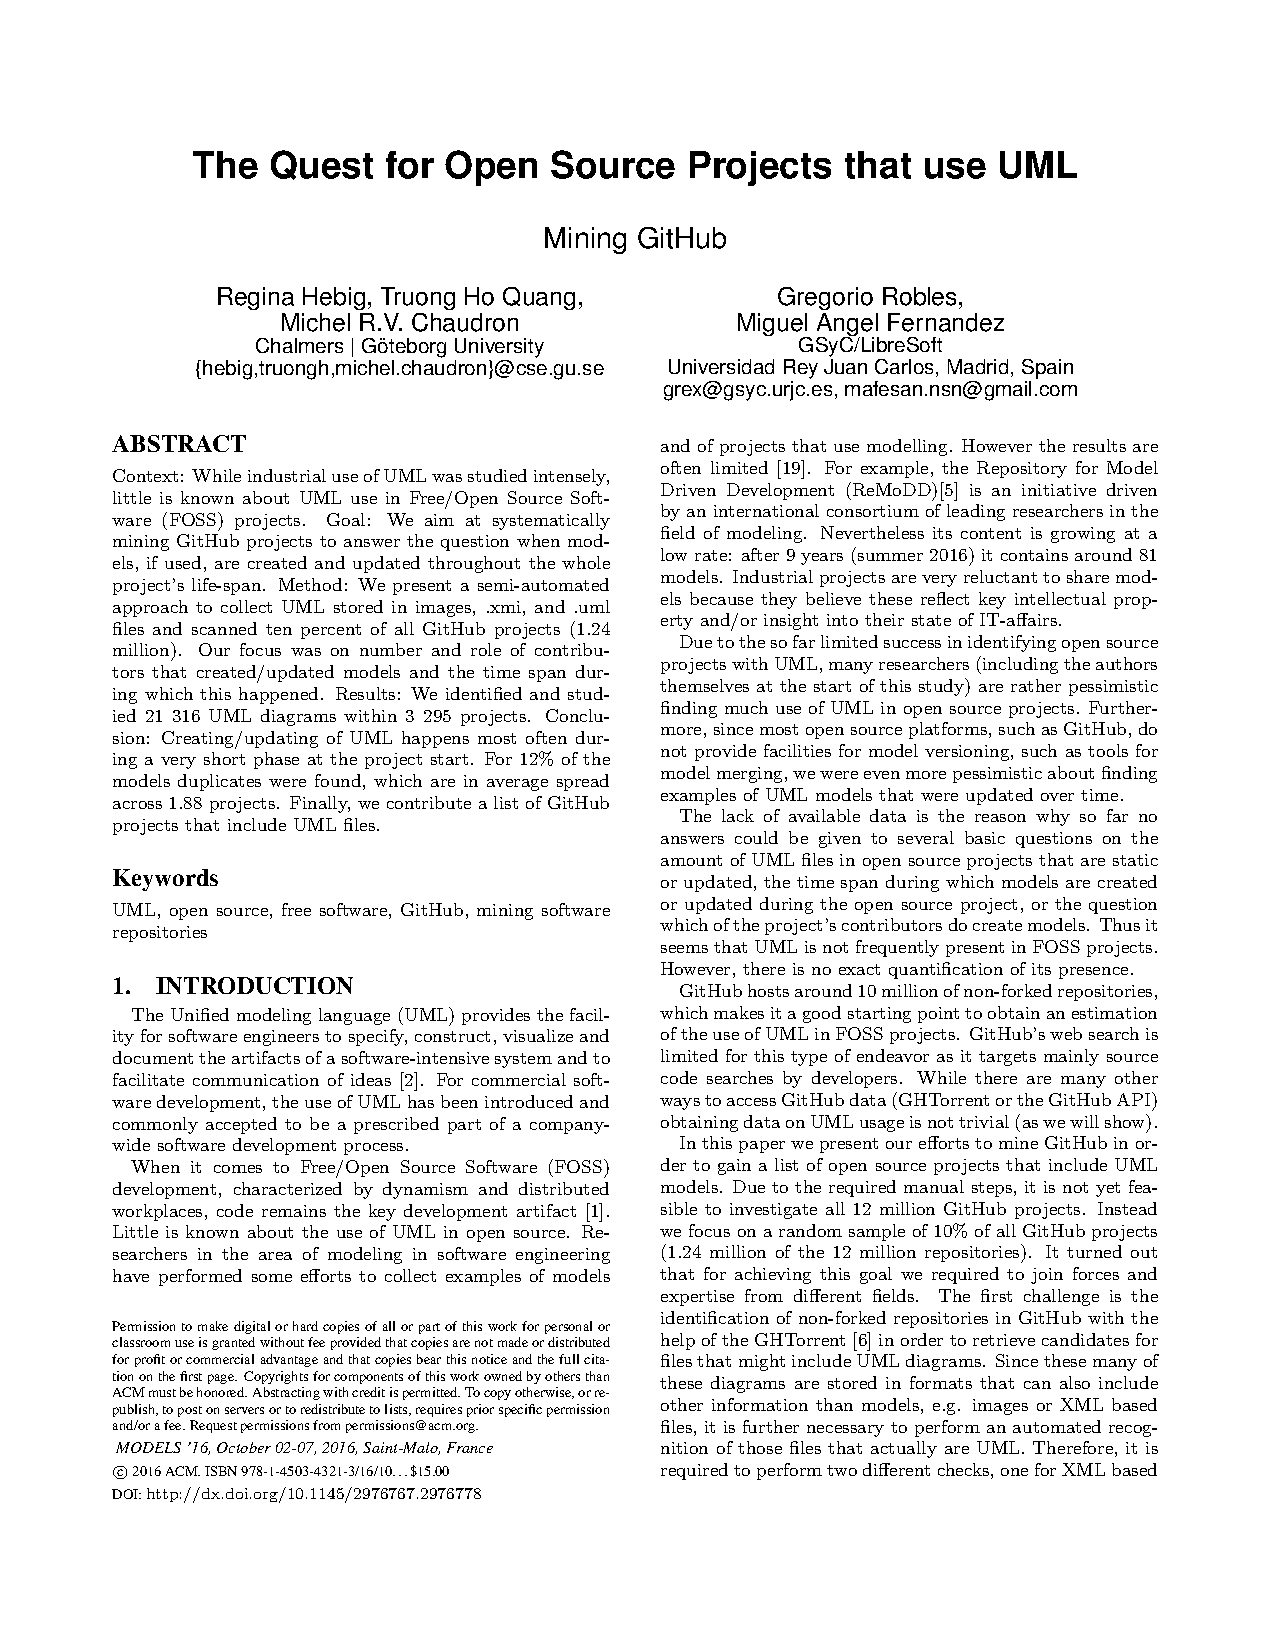
\includepdf[pages=-,pagecommand={},width=1.2\textwidth]{pdf/models.pdf}
%%%%%%%%%%%%%%%%%%%%%%%%%%%%%%%%%%%
\section{An extensive dataset of UML models in GitHub}
\label{sec:paper-msr}
This paper was published in MSR conference (Buenos Aires, Argentina), in May 2017.
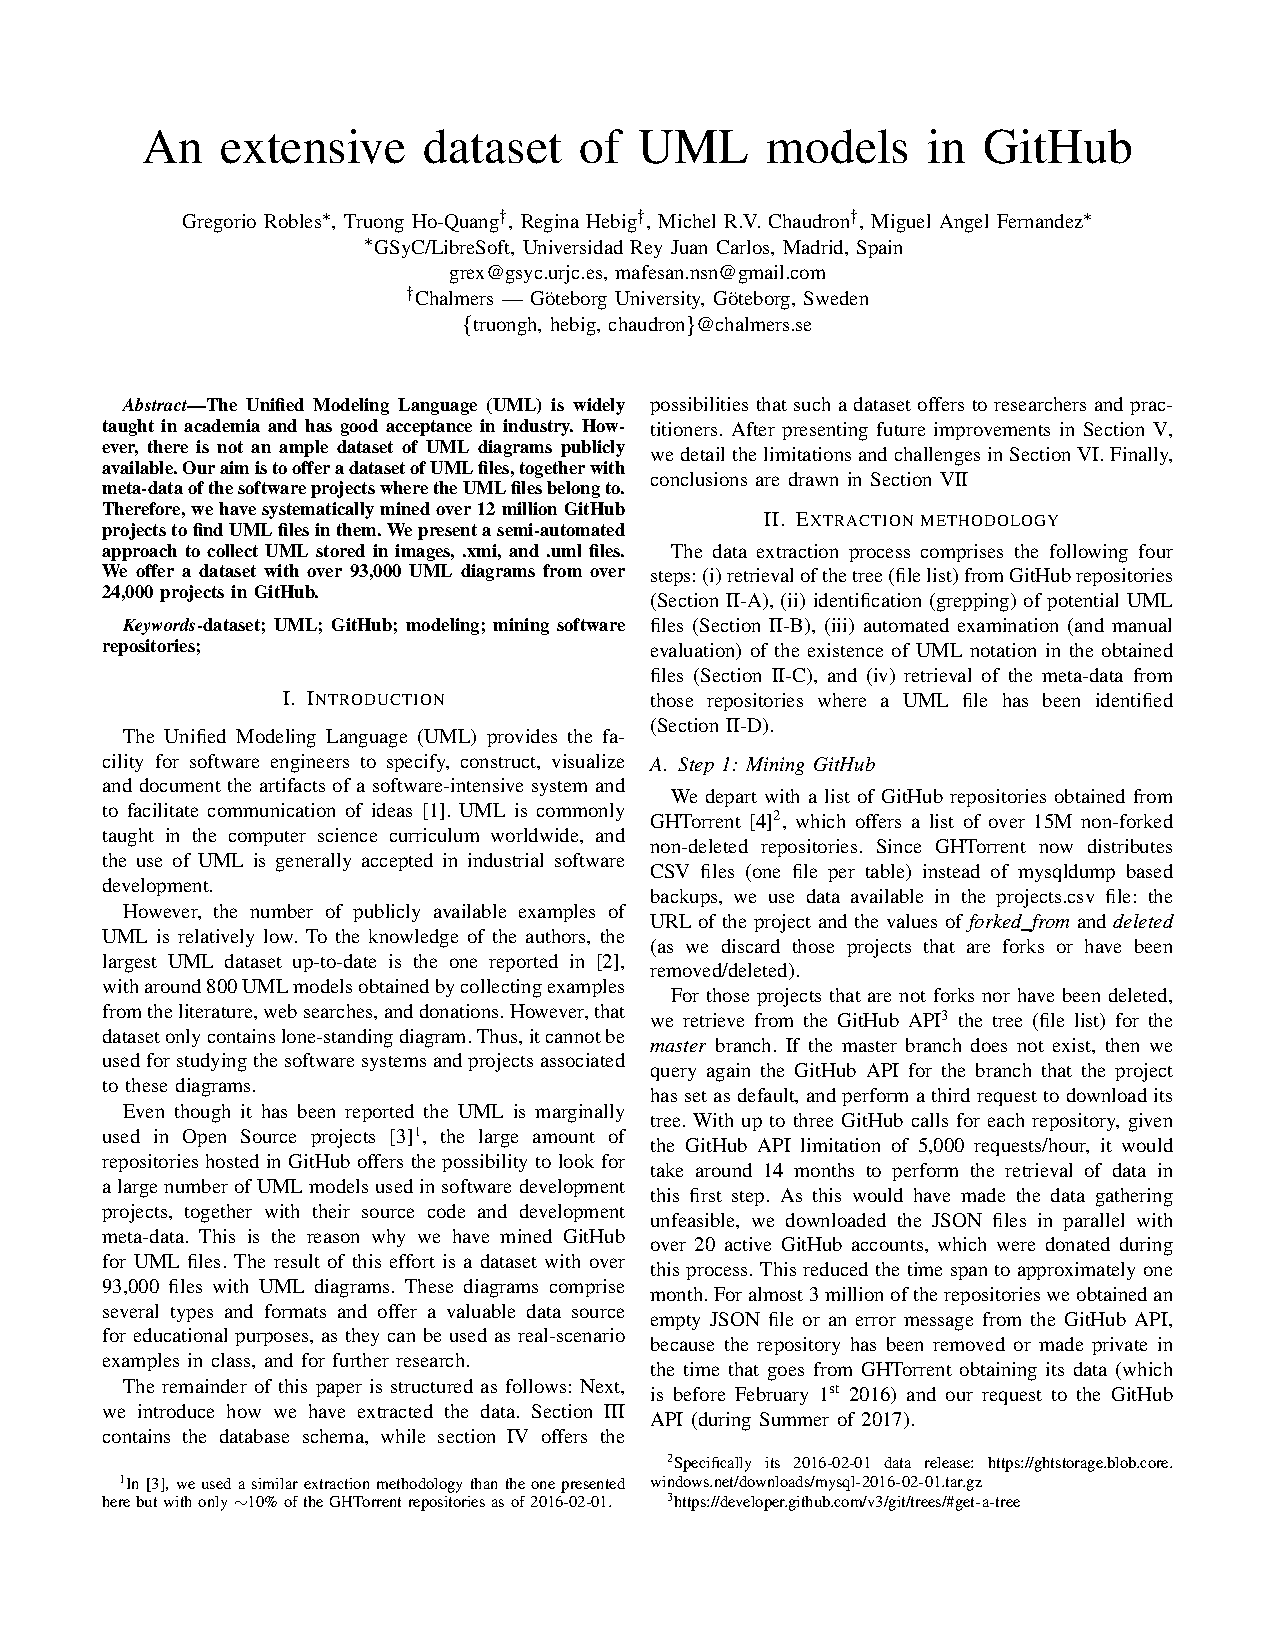
\includepdf[pages=-,pagecommand={},width=1.2\textwidth]{pdf/msr2017.pdf}
%%%%%%%%%%%%%%%%%%%%%%%%%%%%%%%%%%%
\section{Practices and Perceptions of UML Use in OS Projects}
\label{sec:paper-icse}
This paper was published in ICSE-SEIP conference (Buenos Aires, Argentina), in May 2017.
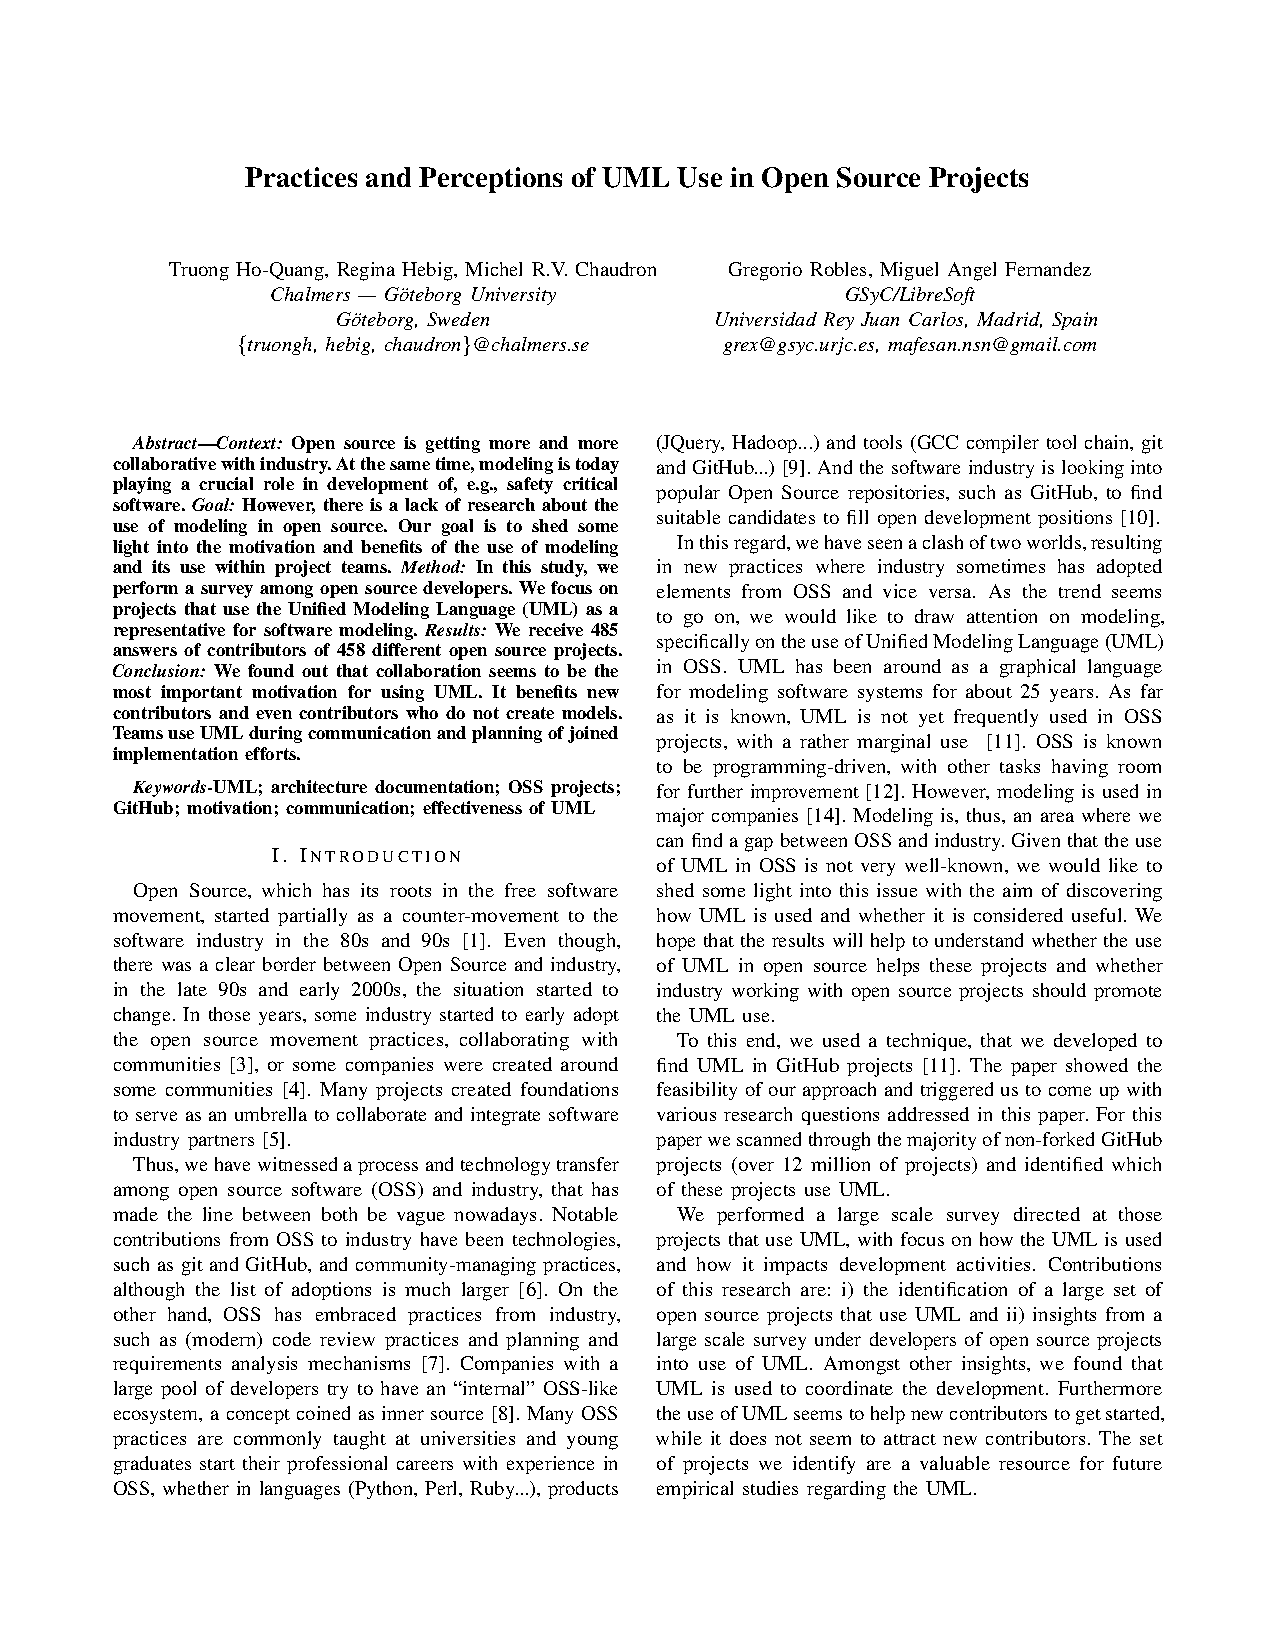
\includepdf[pages=-,pagecommand={},width=1.2\textwidth]{pdf/seip2017.pdf}
%%%%%%%%%%%%%%%%%%%%%%%%%%%%%%%%%%%%%%%%%%%%%%%%%%%%%%%%%%%%%%%%%%%%%%%%%%%%%%%%
%%%%%%%%%%%%%%%%%%%%%%%%%%%%%%%%%%%%%%%%%%%%%%%%%%%%%%%%%%%%%%%%%%%%%%%%%%%%%%%%
% BIBLIOGRAFIA %
%%%%%%%%%%%%%%%%%%%%%%%%%%%%%%%%%%%%%%%%%%%%%%%%%%%%%%%%%%%%%%%%%%%%%%%%%%%%%%%%
\cleardoublepage
% Las siguientes dos instrucciones es todo lo que necesitas
% para incluir las citas en la memoria
\bibliographystyle{abbrv}
\bibliography{memoria}  % memoria.bib es el nombre del fichero que contiene
% las referencias bibliogr�ficas. Abre ese fichero y mira el formato que tiene,
% que se conoce como BibTeX. Hay muchos sitios que exportan referencias en
% formato BibTeX. Prueba a buscar en http://scholar.google.com por referencias
% y ver�s que lo puedes hacer de manera sencilla.
% M�s informaci�n:
% http://texblog.org/2014/04/22/using-google-scholar-to-download-bibtex-citations/
\end{document}
